\documentclass[11pt,twocolumn]{article}

\usepackage[a4paper,top=17mm,bottom=19mm,left=15.5mm,right=15.5mm,columnsep=6.5mm]{geometry}
\usepackage[T1]{fontenc}
\usepackage[utf8]{inputenc}
\usepackage{lmodern}
\usepackage{microtype}
\usepackage{amsmath,amssymb,mathtools}
\usepackage{graphicx}
\usepackage{booktabs}
\usepackage{tabularx}
\usepackage{array}
\usepackage{multirow}
\usepackage{caption}
\usepackage{subcaption}
\usepackage{float}
\usepackage{enumitem}
\usepackage{xcolor}
\usepackage{xspace}
\usepackage{titlesec}
\usepackage{fancyhdr}
\usepackage{natbib}
\usepackage[hidelinks]{hyperref}
\usepackage[nameinlink,noabbrev]{cleveref}

\definecolor{GatesNavy}{HTML}{273746}
\definecolor{GatesBlue}{HTML}{607D98}
\definecolor{GatesTeal}{HTML}{4F8A78}
\definecolor{GatesAmber}{HTML}{B88A32}
\definecolor{GatesRed}{HTML}{A64B45}
\definecolor{GatesRule}{HTML}{D9DEE3}

\graphicspath{{figures/}{../../artifacts/final/figures/}}
\captionsetup{font=small,labelfont={bf,color=GatesNavy},labelsep=period}
\captionsetup[subfigure]{font=footnotesize,labelfont=bf}
\setlength{\parindent}{1em}
\setlength{\parskip}{0pt}
\linespread{1.025}
\setlength{\textfloatsep}{9pt plus 2pt minus 2pt}
\setlength{\floatsep}{8pt plus 2pt minus 2pt}
\setlength{\intextsep}{8pt plus 2pt minus 2pt}
\setlist[itemize]{leftmargin=1.35em,itemsep=1pt,topsep=3pt}
\setlist[enumerate]{leftmargin=1.45em,itemsep=1pt,topsep=3pt}
\titleformat{\section}{\large\bfseries\color{GatesNavy}}{\thesection}{0.55em}{}
\titleformat{\subsection}{\normalsize\bfseries\color{GatesNavy}}{\thesubsection}{0.5em}{}
\titlespacing*{\section}{0pt}{11pt}{5pt}
\titlespacing*{\subsection}{0pt}{8pt}{3pt}
\renewcommand{\arraystretch}{1.12}
\pagestyle{fancy}
\setlength{\headheight}{22pt}
\fancyhf{}
\fancyhead[L]{\footnotesize\color{GatesBlue}GATES: Group-Aware Time-Efficient Stopping}
\fancyhead[R]{\footnotesize\color{GatesBlue}Atharva Parande}
\fancyfoot[C]{\footnotesize\thepage}
\renewcommand{\headrulewidth}{0.3pt}
\renewcommand{\headrule}{\hbox to\headwidth{\color{GatesRule}\leaders\hrule height \headrulewidth\hfill}}
\hypersetup{
  colorlinks=true,
  linkcolor=GatesNavy,
  citecolor=GatesTeal,
  urlcolor=GatesBlue,
  pdftitle={GATES: Group-Aware Time-Efficient Stopping for Longitudinal Biological Experiments},
  pdfauthor={Atharva Parande}
}

\newcommand{\method}{\textsc{Gates}\xspace}
\newcommand{\eesr}{\mathrm{EESR}}
\newcommand{\stopstate}{\textsc{Stop}\xspace}
\newcommand{\continuestate}{\textsc{Continue}\xspace}
\newcommand{\abstainstate}{\textsc{Abstain}\xspace}
\newcommand{\pct}[1]{#1\%}

\title{\vspace{-1.4em}\textbf{GATES: Group-Aware Time-Efficient Stopping\\for Longitudinal Biological Experiments}}
\author{Atharva Parande}
\date{September 2026}

\begin{document}
\maketitle
\thispagestyle{fancy}

\begin{abstract}
Longitudinal biological experiments are commonly observed on fixed schedules even when their
endpoints become predictable earlier. Prediction alone, however, does not establish that continued
measurement is unnecessary: confidence can fail under experiment-to-experiment heterogeneity.
We introduce \method, an experiment-disjoint selective-stopping framework that asks whether the
available prefix of a trajectory justifies an early endpoint decision. \method combines
prefix-based prediction, calibration on independent biological experiments, a feature-distance
refusal check, and sequential \stopstate, \continuestate, or \abstainstate actions. We evaluate the
complete frozen policy retrospectively on 988 medaka retinal organoids from 11 independent
experiments, comprising 114,510 released longitudinal morphometric observations through 72 h. At
the frozen operating point, \method made 439 early decisions with 25 errors: a \pct{5.69} observed
held-out erroneous-early-stop rate (exact unit-level 95\% confidence interval,
\pct{3.72}--\pct{8.29}), \pct{44.43} coverage, and \pct{12.26} retrospectively estimated
observation savings. Removing refusal increased observed error to \pct{8.60} while increasing
estimated savings to \pct{13.65}. The aggregate result conceals substantial heterogeneity: one
held-out experiment reached \pct{30.61} error among early stops, and experiment-bootstrap
uncertainty is wide. These findings are promising retrospective evidence, not an anytime-valid or
deployment guarantee. \method provides an auditable formulation for converting longitudinal
prediction into a decision about whether another measurement remains necessary.
\end{abstract}

\section{Introduction}

Longitudinal biological studies often follow fixed acquisition schedules: images or measurements
are collected repeatedly until a predetermined endpoint, even when the available trajectory may
already contain useful endpoint information. Earlier decisions could reduce acquisition burden,
microscope occupancy, storage, and downstream analysis for selected experimental units. A
prematurely wrong decision, however, can corrupt the study by stopping observation before the true
endpoint is known. The relevant problem is therefore not simply early prediction; it is deciding
when an early prediction is reliable enough to justify termination.

This distinction is especially important in biology. Measurements are nested within experimental
units, which are themselves nested within batches or experiments. A classifier can perform well in
aggregate while failing severely in one held-out experiment. Confidence estimated without
respecting this hierarchy may therefore be unsuitable for an intervention such as stopping.
Experimental groups are not merely train--test bookkeeping: experiment-to-experiment variation is
part of the reliability problem.

\method frames observation as a sequential selective decision. At each candidate time, it uses
only the available trajectory prefix, estimates the eventual binary endpoint, checks calibrated
confidence and familiarity, and returns \stopstate, \continuestate, or \abstainstate. The policy is
evaluated as a whole on experiments excluded from fitting, calibration, and refusal-threshold
selection. Its principal outputs are erroneous early-stop rate, coverage, and retrospectively
estimated observation savings, reported across complete risk--savings and risk--coverage
frontiers rather than as a single accuracy value.

Our contributions are:
\begin{itemize}
  \item an experiment-disjoint formulation of selective stopping for longitudinal biological
        endpoints;
  \item independent-group confidence calibration coupled to explicit trajectory-level refusal;
  \item evaluation through risk--coverage--savings tradeoffs with unit- and experiment-level
        uncertainty; and
  \item a reproducible decision record that retains negative transfer, robustness failures, and
        severe experiment-specific errors.
\end{itemize}

\begin{figure*}[t]
  \centering
  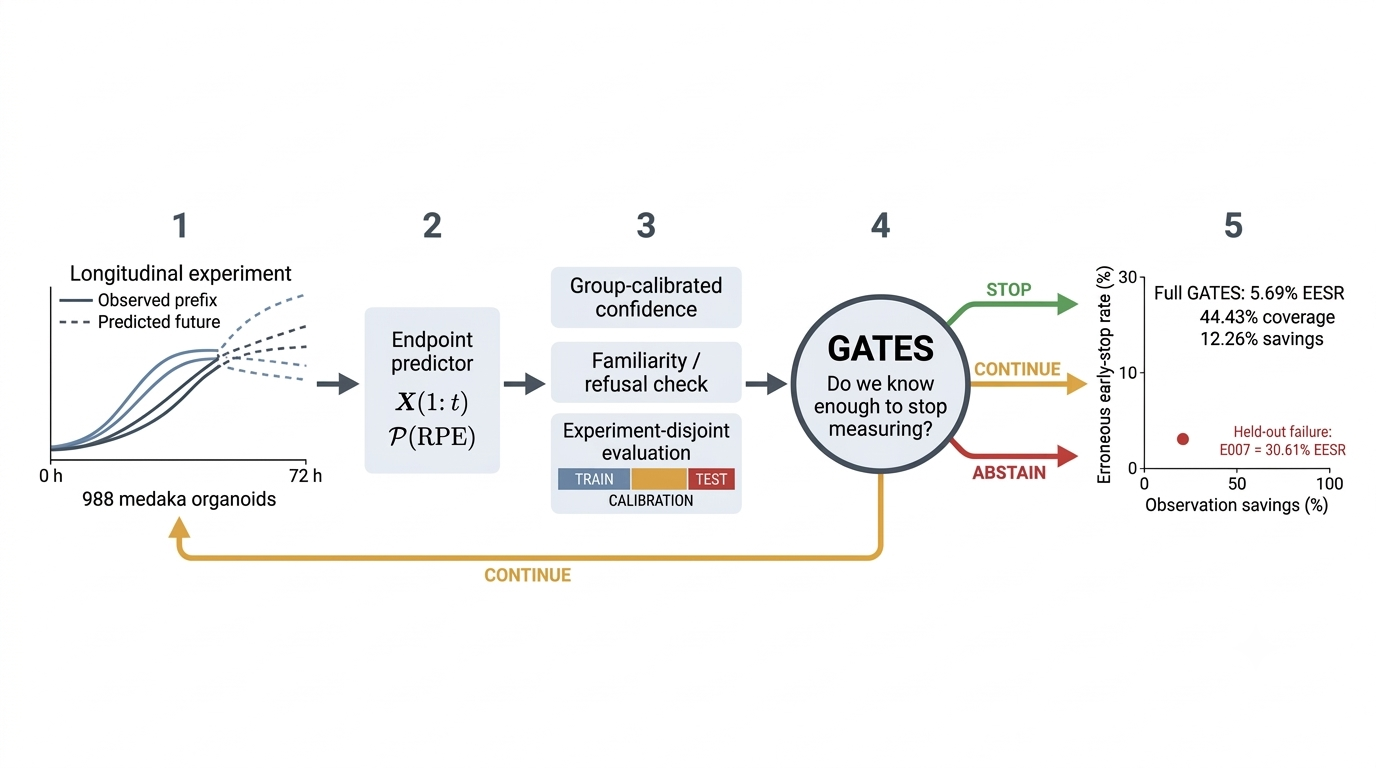
\includegraphics[width=0.98\textwidth]{gates_overview.png}
  \caption{Overview of \method. Partial longitudinal trajectories are converted into endpoint
  predictions, calibrated using independent experimental groups, and passed through a refusal
  mechanism before a sequential \stopstate, \continuestate, or \abstainstate decision. Evaluation
  is performed on completely held-out experiments and summarized through the tradeoff between
  premature-decision risk and retrospectively estimated observation savings.}
  \label{fig:overview}
\end{figure*}

\section{Related work}

\paragraph{Early classification and selective prediction.}
Early classification of time series studies the tradeoff between predictive accuracy and decision
earliness, including rules for selecting a useful prefix \citep{xing2012early}. Selective
prediction and reject-option learning permit abstention so that risk is measured on the covered
subset \citep{geifman2019selectivenet}. \method draws on both traditions, but treats complete
biological experiments as the calibration and generalization boundary and measures the downstream
cost of continued observation.

\paragraph{Calibration and risk control.}
Conformal prediction and conformal risk control provide rigorous uncertainty or risk statements
under explicit assumptions \citep{angelopoulos2023gentle,angelopoulos2024crc}. The current \method
policy is not conformal and does not provide distribution-free, anytime-valid, or
group-conditional risk control. Its observed held-out rate is an empirical property of the
complete frozen sequential procedure.

\paragraph{Experimental stopping.}
Confidence-bound early stopping (CBES) is the closest prior experimental-stopping method
\citep{liu2026cbes}. CBES combines probabilistic prediction, confidence bounds, sequential
calibration, and a Hoeffding-based validation bound in its own setting. We do not claim a stronger
formal result. The comparator used here is a documented binary adaptation: bootstrap logistic
ensembles replace the original continuous Gaussian-process model, and symmetric bounds around 0.5
define the two endpoint decisions. Both receive the same features, candidate times, and held-out
experiments. This is not a byte-for-byte reproduction of all CBES formulations.

\paragraph{Biological heterogeneity.}
Technical and biological batch effects can invalidate naive generalization
\citep{leek2010batch}. Reporting standards for supervised learning in biology similarly emphasize
separation of development and evaluation data, transparent optimization, and appropriate metrics
\citep{walsh2021dome}. The source orgAInoid work established early outcome prediction from retinal
organoid morphology \citep{afting2026orgainoid}; \method addresses the downstream question of
whether a specific partial trajectory justifies terminating observation.

\section{Dataset and biological context}

We use the CC BY 4.0 source data released by \citet{afting2026orgainoid}. The biological system is
\emph{Oryzias latipes} (medaka) retinal organoids, not human organoids. The study contains 988
organoid wells from 11 independent experiments, imaged every 30 minutes for up to 72 h. The final
morphology label for retinal pigment epithelium (RPE) formation is the primary binary endpoint;
Lens formation is retained as a transfer analysis.

\begin{table}[t]
\centering
\caption{Dataset and evaluation hierarchy. Observations are not independent biological units.}
\label{tab:hierarchy}
\small
\begin{tabularx}{\columnwidth}{@{}>{\raggedright\arraybackslash}X r@{}}
\toprule
Released morphometric observations & 114,510 \\
Organoid wells (prediction units) & 988 \\
Independent experiments (holdout units) & 11 \\
Maximum observation horizon & 72 h \\
RPE positive / negative & 405 / 583 \\
Lens positive / negative & 450 / 538 \\
Complete 144-observation trajectories & 381 \\
Trajectories with fewer than 72 observations & 189 \\
Trajectories with fewer than 12 observations & 85 \\
\bottomrule
\end{tabularx}
\end{table}

The hierarchy is 114,510 longitudinal observations nested within 988 organoid wells, themselves
nested within 11 experiments. An organoid well is the prediction unit; an experiment is the
generalization and resampling boundary. Availability variables are excluded from predictors
because they can encode experiment identity.

\subsection{Reconciling image and morphometric counts}

The source article reports 117,249 acquired images, whereas \method uses exactly 114,510 released
morphometric rows. These counts describe different objects. The pipeline pins and reads
\texttt{Extended\_Data\_2.csv}, the publication's released morphometrics table. Audit and modeling
loaders select columns but remove no rows. The difference of 2,739 therefore arose upstream,
between acquisition and the published table. Neither the article nor the table gives per-image
exclusion reasons; no specific cause, such as segmentation failure, is inferred.

\section{Problem formulation}

For organoid $i$, let $X_{i,1:t}$ denote the measurements available up to candidate time $t$, and
let $y_i\in\{0,1\}$ be its final endpoint at horizon $T=72$ h. A predictor produces
$p_{i,t}=\Pr(y_i=1\mid X_{i,1:t})$ and label
\begin{equation}
  \widehat y_{i,t}=\mathbb{1}[p_{i,t}\geq 1/2].
\end{equation}
The sequential policy selects a terminal action
$a_{i,t}\in\{\stopstate,\continuestate,\abstainstate\}$ and an associated decision time
$\tau_i$. An erroneous early stop occurs if
\begin{equation}
  \tau_i<T \quad\land\quad \widehat y_{i,\tau_i}\neq y_i.
\end{equation}
Let $S_i=\mathbb{1}[\tau_i<T\ \land\ a_{i,\tau_i}=\stopstate]$. The erroneous early-stop rate is
\begin{equation}
  \eesr=
  \frac{\sum_{i=1}^{n} S_i\,\mathbb{1}[\widehat y_{i,\tau_i}\neq y_i]}
       {\sum_{i=1}^{n} S_i}.
  \label{eq:eesr}
\end{equation}
Coverage is the fraction of units stopped early,
\begin{equation}
  \mathrm{Coverage}=\frac{1}{n}\sum_{i=1}^{n}S_i.
\end{equation}
If $m_i(T)$ is the number of scheduled observations available through the endpoint and
$m_i(\tau_i)$ the number consumed by the policy, retrospective observation savings are
\begin{equation}
  \mathrm{Savings}=\frac{1}{n}\sum_{i=1}^{n}
  S_i\left(1-\frac{m_i(\tau_i)}{m_i(T)}\right).
  \label{eq:savings}
\end{equation}
This quantity estimates observations that would not have been required after a frozen early stop;
it is not observed microscope time, laboratory duration, monetary cost, or prospective resource
savings.

\section{GATES method}

\Cref{fig:overview} summarizes the complete decision path. At each candidate time, leakage-safe
prefix features summarize only measurements available by that time. A regularized classifier
estimates the endpoint probability. Identifiers, availability variables, and final labels are
excluded from predictor features.

\subsection{Independent-group calibration}

Training, preprocessing, confidence calibration, and refusal-threshold fitting exclude the
complete held-out experiment. Development experiments calibrate confidence thresholds for the
requested operating point. If confidence does not pass, the action is \continuestate. The 5\%
label is a calibration target, not certified risk control.

\subsection{Familiarity and refusal}

A training-derived feature-distance score compares the current prefix with the fitted reference
distribution. If the score exceeds its frozen threshold, the policy returns \abstainstate and
observes the unit through the endpoint. Otherwise, a sufficiently confident endpoint call returns
\stopstate. The refusal score is a limited diagnostic for generic feature-space distance; it does
not prove that every shifted experiment will be detected.

\subsection{Sequential decision contract}

Repeated looks occur at the candidate times of the frozen policy. \stopstate commits to an early
endpoint prediction, \continuestate requests further observation, and \abstainstate disables early
automation for that trajectory. Because the procedure does not construct an anytime-valid
confidence sequence, Eq.~\eqref{eq:eesr} remains an empirical held-out metric for the full
sequential policy.

\section{Experiment-disjoint evaluation}

Eleven rotations hold out one complete experiment at a time. Every well, frame, prefix, and label
from that experiment is excluded from model fitting and rule selection. All prefixes from a well
remain inside the same experiment. The rotations yield exactly one held-out terminal decision for
each of 988 organoids.

Unit-level EESR receives a two-sided Clopper--Pearson interval. To reflect variation at the actual
generalization boundary, aggregate metrics also receive a 10,000-draw percentile bootstrap over
the 11 held-out experiments. The experiment-level interval is necessarily wide and is more
relevant to between-experiment transfer than the unit-level binomial interval alone.

\section{Baselines}

The frozen comparison includes full observation, fixed stopping times, naive confidence,
non-group calibration, a CBES-style adaptation, \method without refusal, and Full \method. Each
method is evaluated on the same held-out experiments. Fixed time applies one decision time to all
eligible trajectories. Naive confidence uses uncalibrated predictive confidence. Non-group
calibration pools development units without preserving experiments as calibration groups. The
CBES-style comparator uses sequential calibration and validation roles as described above. Full
\method adds experiment-aware calibration and trajectory-level refusal.

No single scalar ranking is adequate because the methods stop different numbers of organoids at
different times. Risk--savings and risk--coverage frontiers are therefore the primary comparison
(\cref{fig:frontiers}).

\begin{figure*}[t]
  \centering
  \begin{subfigure}[t]{0.495\textwidth}
    \centering
    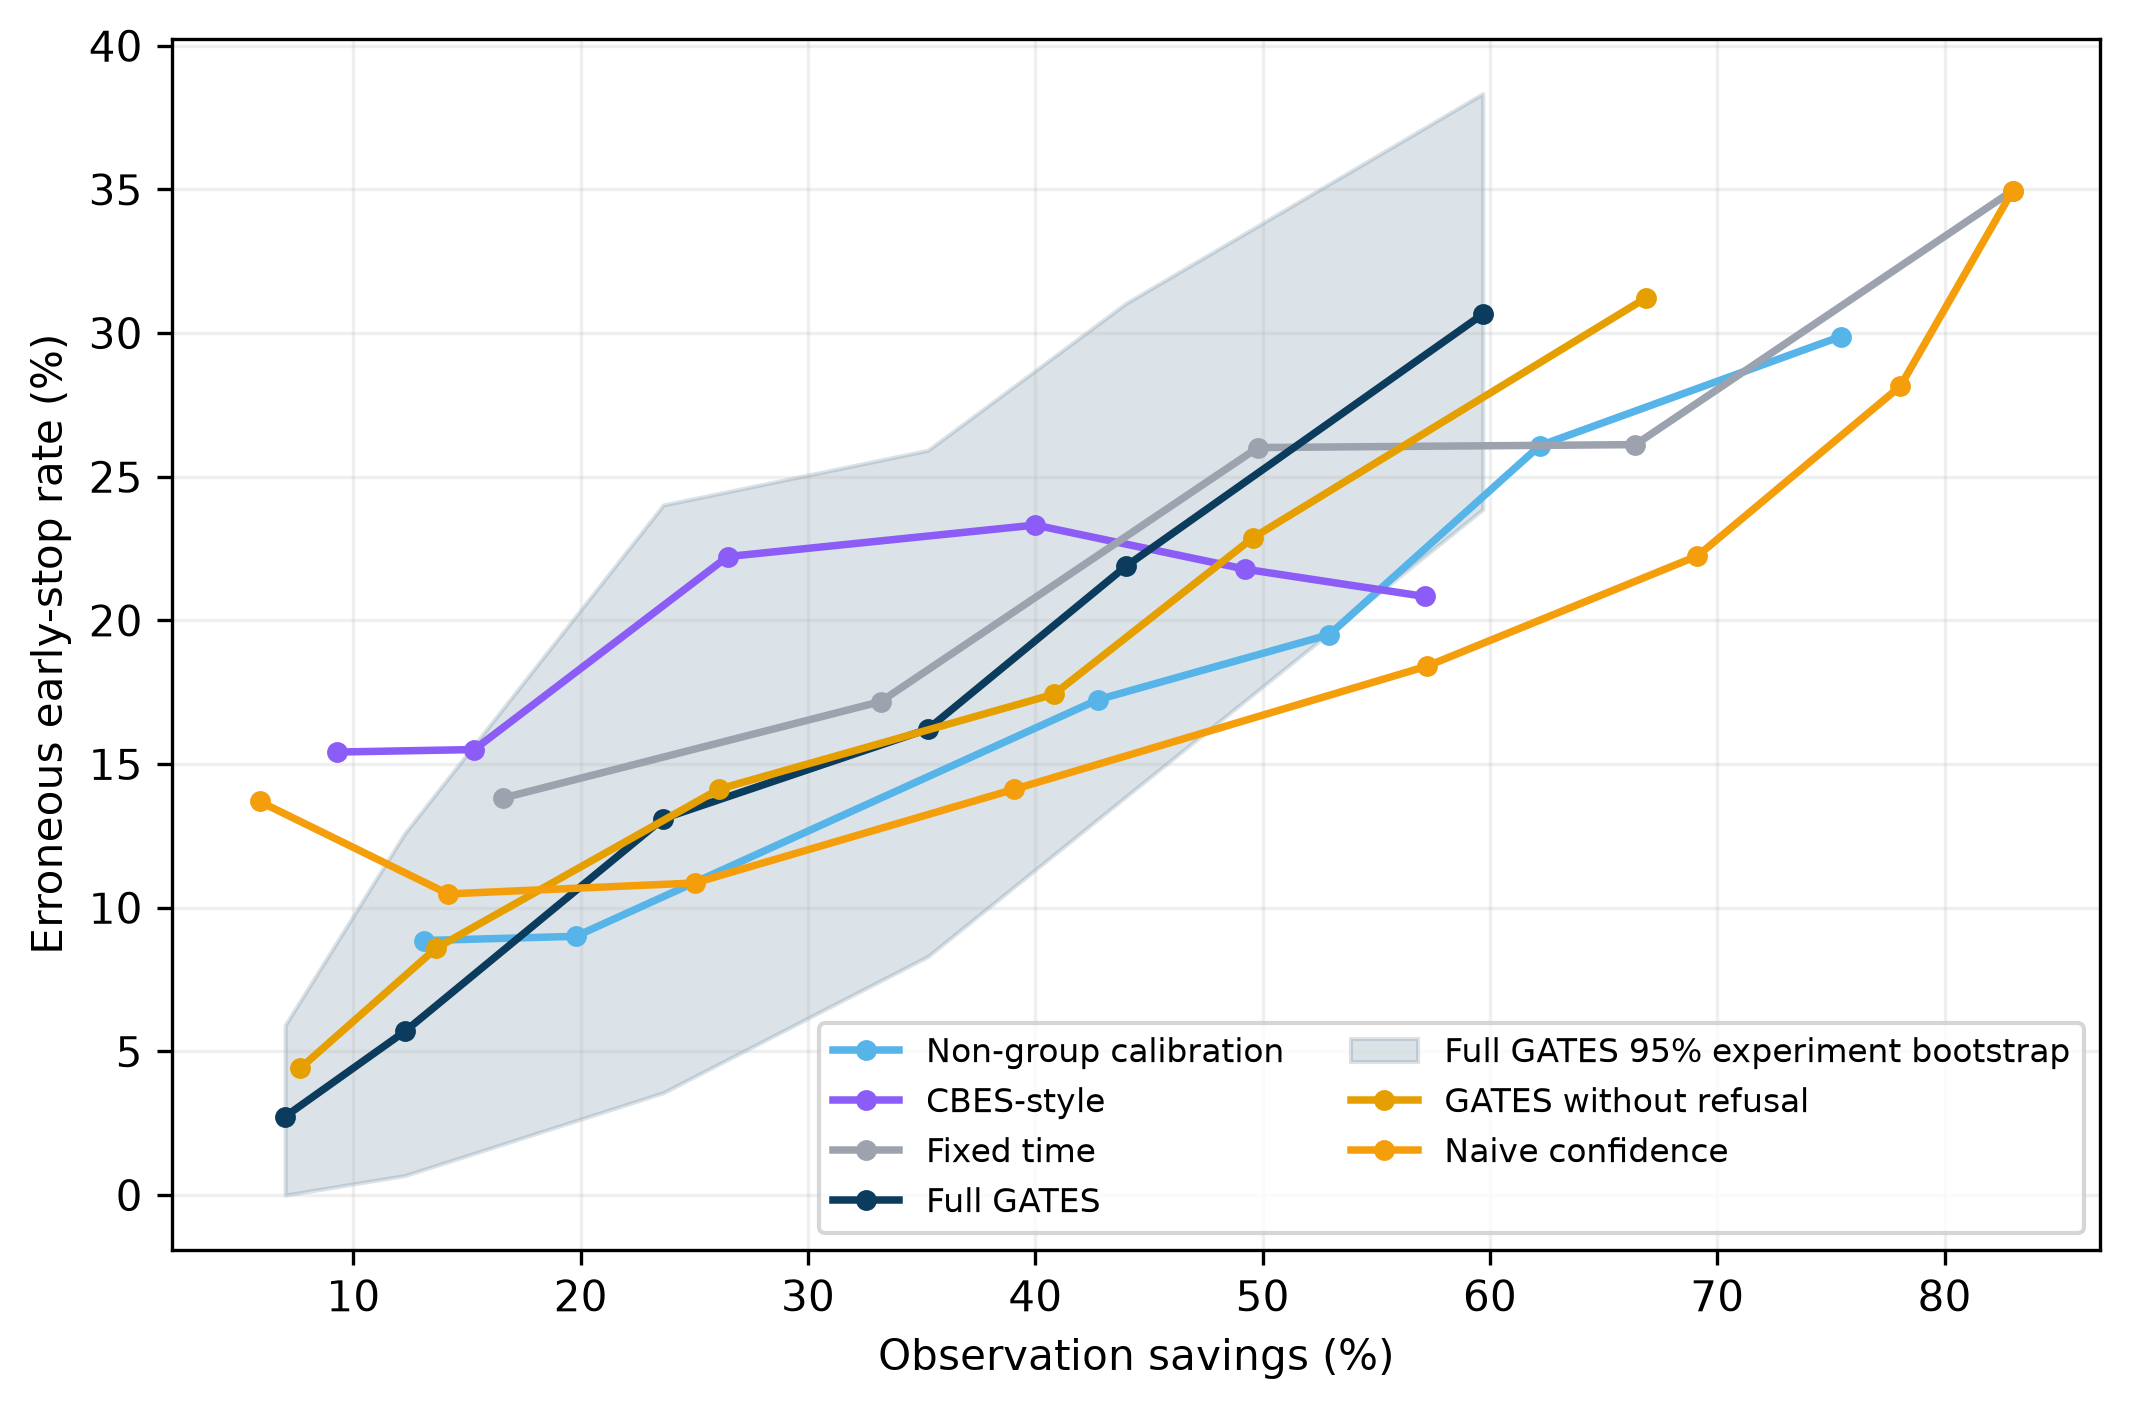
\includegraphics[width=\linewidth]{01_rpe_risk_savings_frontier.png}
    \caption{Observed EESR versus retrospectively estimated observation savings.}
  \end{subfigure}\hfill
  \begin{subfigure}[t]{0.495\textwidth}
    \centering
    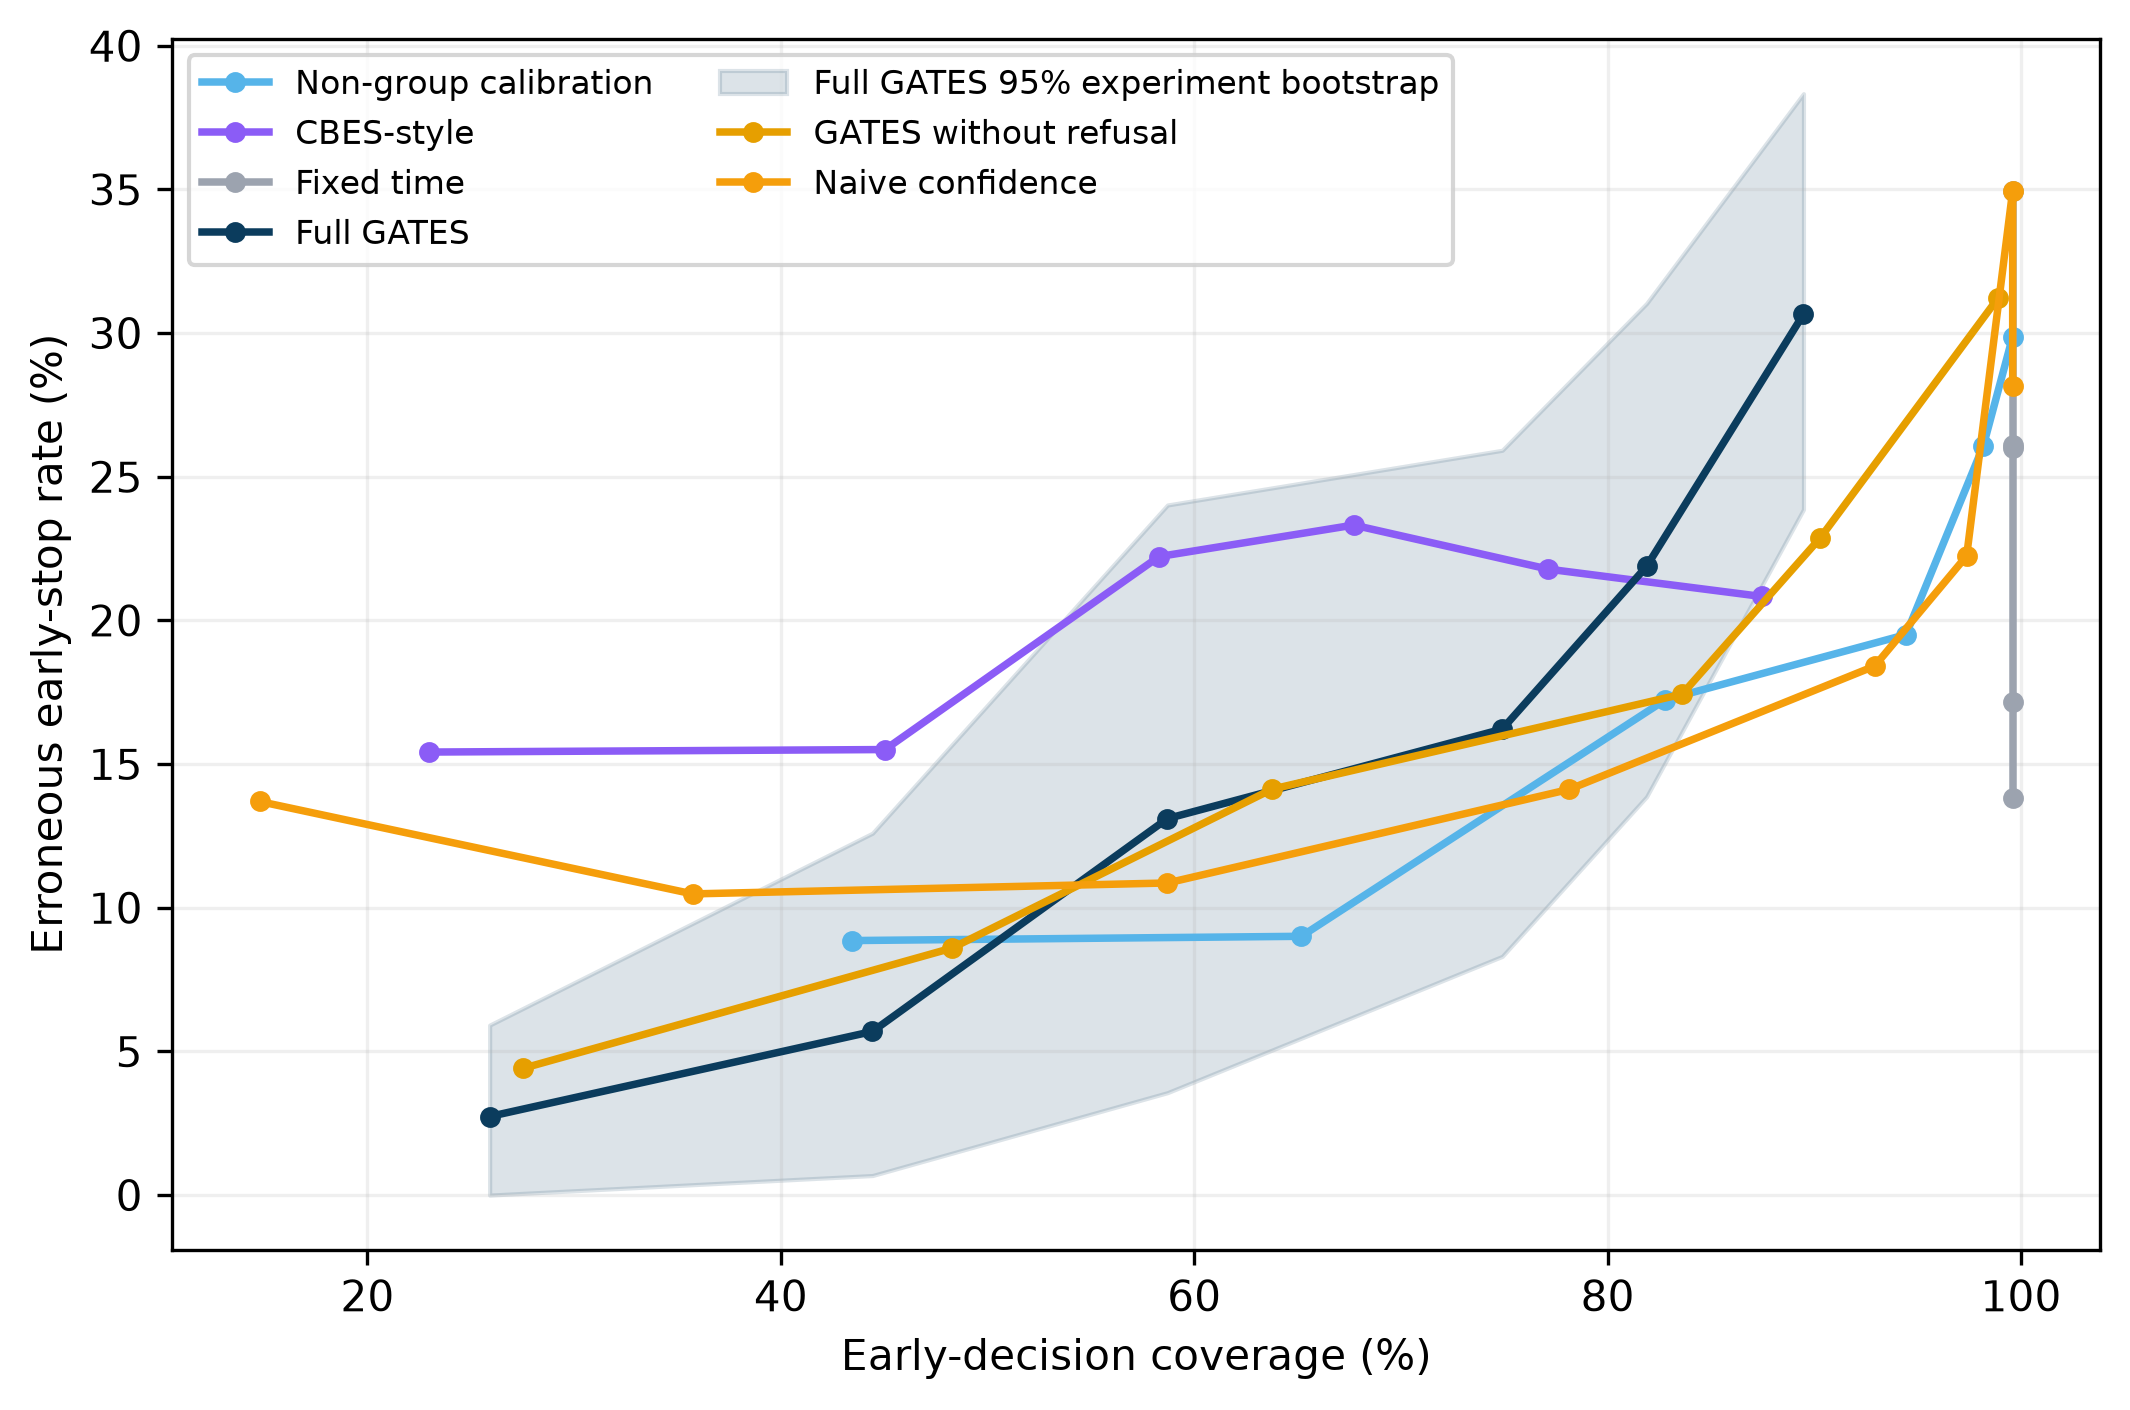
\includegraphics[width=\linewidth]{02_rpe_risk_coverage_frontier.png}
    \caption{Observed EESR versus early-decision coverage.}
  \end{subfigure}
  \caption{Frozen RPE operating frontiers across 11 experiment-held-out rotations. Marker shape,
  line style, and color distinguish methods. The emphasized Full \method point is the frozen 5\%
  operating point. Methods occupy different coverage and savings regimes, so the tradeoff surface,
  rather than a single bar, is the appropriate comparison.}
  \label{fig:frontiers}
\end{figure*}

\section{Main results}

At the frozen 5\% operating point, Full \method stopped 439 of 988 organoids and made 25 errors.
Observed held-out EESR was \pct{5.69} (unit-level exact 95\% confidence interval,
\pct{3.72}--\pct{8.29}), coverage was \pct{44.43}, abstention was \pct{3.85}, and retrospective
observation savings were \pct{12.26}. Experiment-bootstrap intervals were
\pct{0.68}--\pct{12.60} for EESR, \pct{27.06}--\pct{61.52} for coverage, and
\pct{6.74}--\pct{17.98} for savings. The contrast between the unit-level interval and the wider
experiment bootstrap underscores that the 114,510 observations are not independent evidence for
cross-experiment generalization.

\begin{table*}[t]
\centering
\caption{Frozen RPE comparison at the selected 5\% operating point. Values describe different
risk--coverage--savings tradeoffs and should not be read as a simple accuracy ranking.}
\label{tab:main}
\small
\begin{tabular}{@{}lrrrr@{}}
\toprule
Method & Early stops & Errors & EESR & Coverage / savings \\
\midrule
Safest tested fixed time & 984 & 136 & 13.82\% & 99.60\% / 16.60\% \\
Naive confidence & 643 & 67 & 10.48\% & 65.08\% / 14.17\% \\
Non-group calibration & 644 & 58 & 9.01\% & 65.18\% / 19.79\% \\
CBES-style adaptation & 445 & 69 & 15.51\% & 45.04\% / 15.32\% \\
\method\ without refusal & 477 & 41 & 8.60\% & 48.28\% / 13.65\% \\
\textbf{Full \method} & \textbf{439} & \textbf{25} & \textbf{5.69\%} & \textbf{44.43\% / 12.26\%} \\
\bottomrule
\end{tabular}
\end{table*}

At this point, \method permits early automation for \pct{44.43} of organoids and deliberately
continues observation for the remainder rather than forcing a premature decision. At the frozen
10\% point, coverage and savings increased to \pct{58.70} and \pct{23.63}, respectively, while
observed EESR increased to \pct{13.10}. Coverage is therefore an operating characteristic, not the
fraction on which prediction ``works.''

\section{Refusal ablation}

Without refusal, \method made 477 early decisions with 41 errors, corresponding to \pct{8.60}
EESR and \pct{13.65} savings. With refusal, it made 439 early decisions with 25 errors,
corresponding to \pct{5.69} EESR and \pct{12.26} savings (\cref{fig:refusal}). Thus, under the
frozen RPE evaluation, refusal reduced observed premature error while sacrificing 1.39 percentage
points of estimated observation savings. The effect is operational rather than decorative, but it
does not establish general OOD detection: the unit-level gate missed the important E007 and E012
failure modes.

\begin{figure}[t]
  \centering
  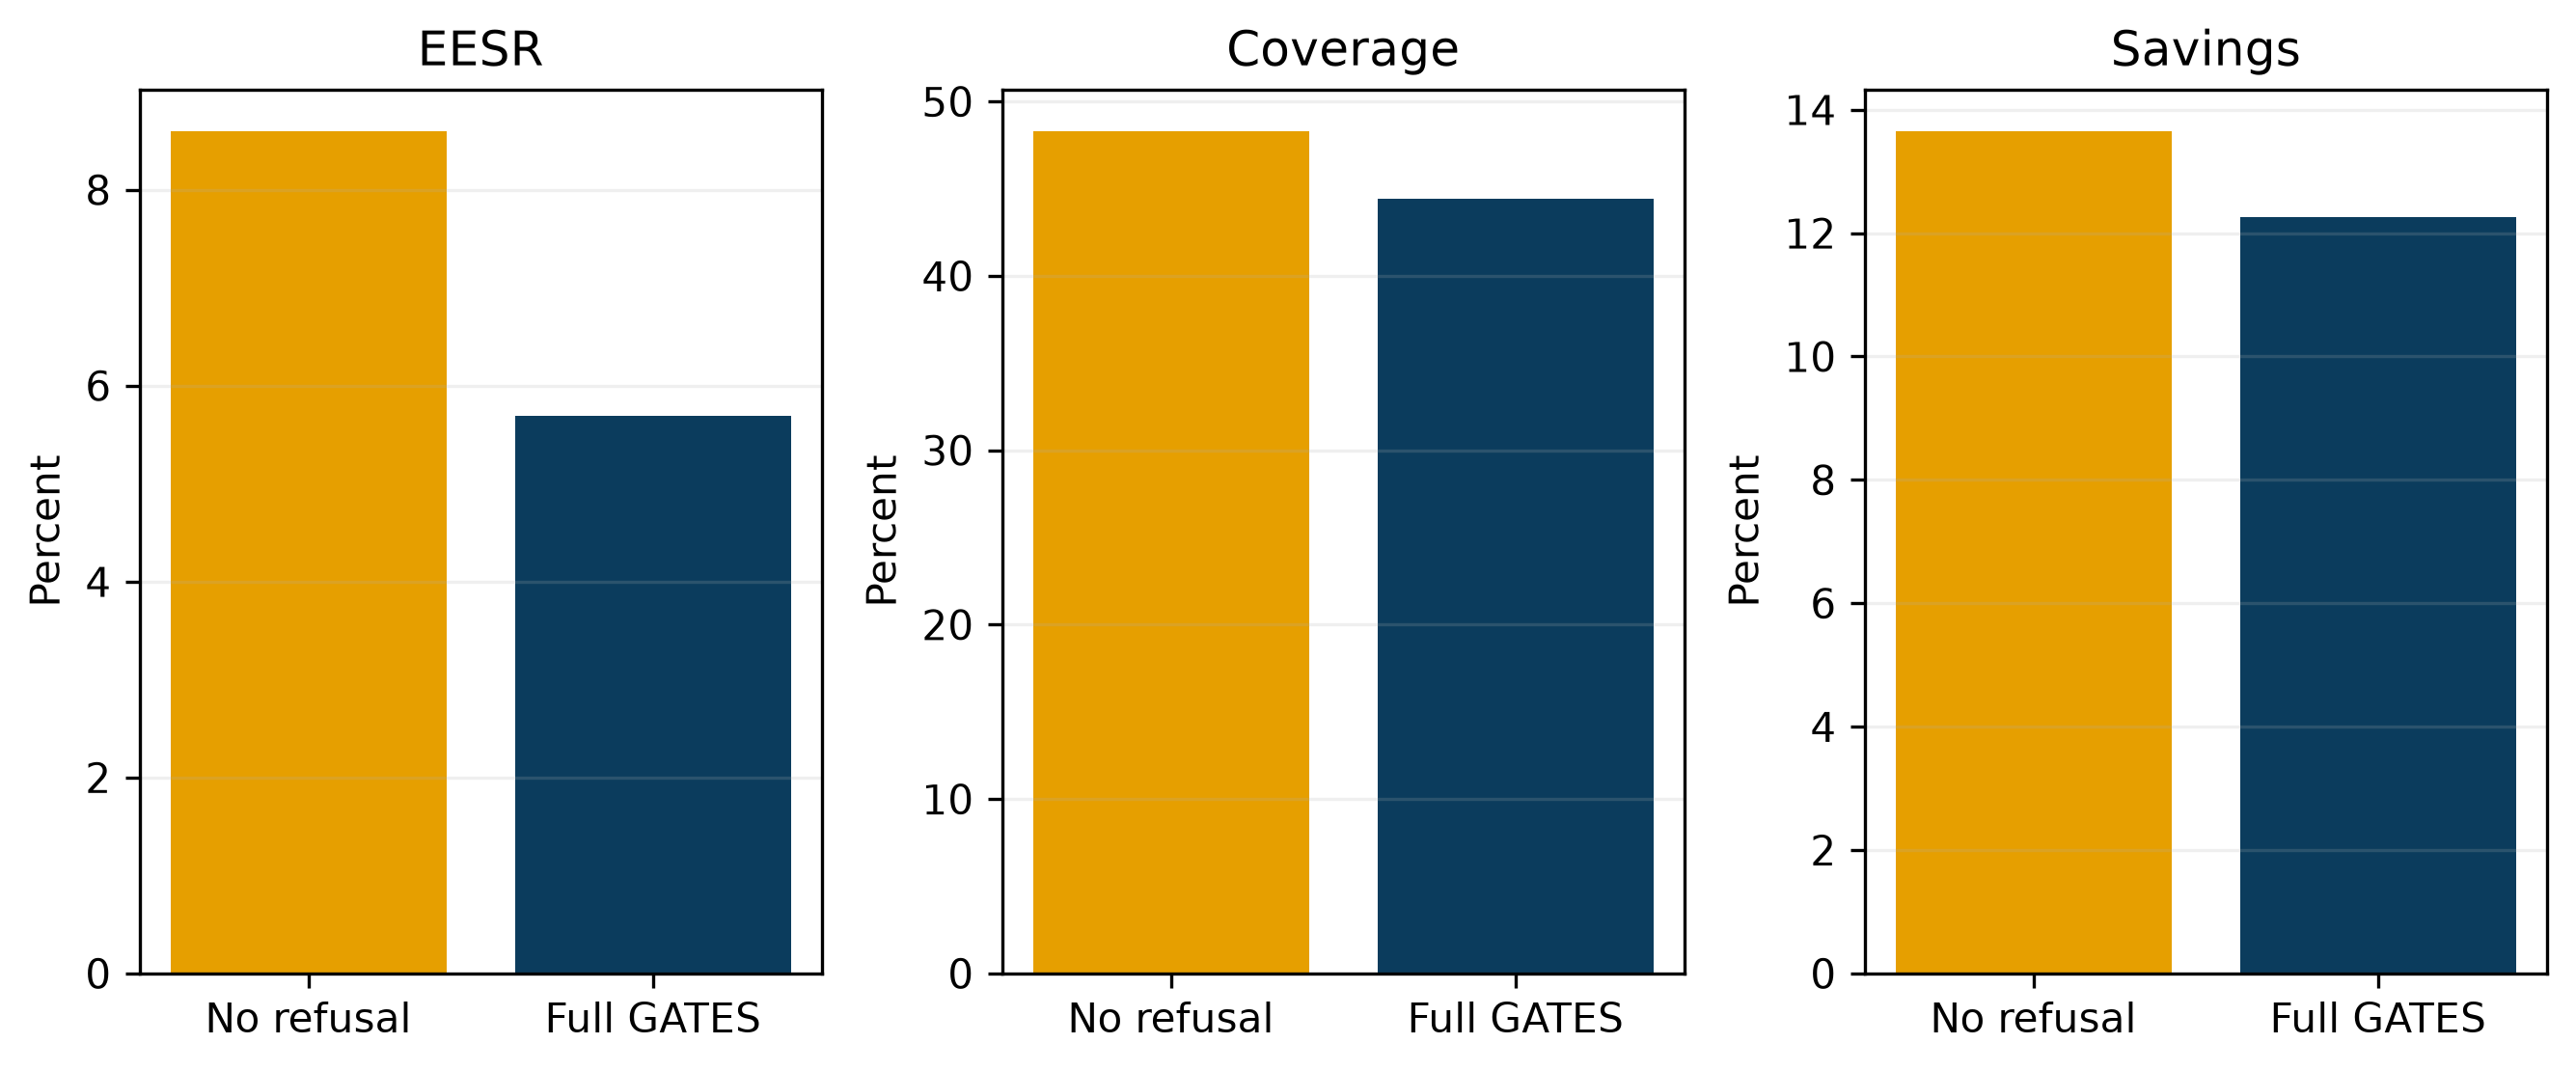
\includegraphics[width=\columnwidth]{06_ood_refusal_ablation.png}
  \caption{Refusal ablation on frozen held-out RPE decisions. Adding the feature-distance refusal
  check reduced errors from 41/477 to 25/439 while estimated savings changed from \pct{13.65} to
  \pct{12.26}. Both risk and retained coverage are reported to avoid rewarding rejection alone.}
  \label{fig:refusal}
\end{figure}

\section{Experiment-level heterogeneity}

Seven held-out experiments had zero early-stop errors; E007, E008, E009, and E012 did not
(\cref{fig:heterogeneity}). E007 contributed 15 errors among 49 early stops (\pct{30.61} EESR),
including five false positives and ten false negatives at 24, 48, and 60 h. Generic
feature-distance statistics were not extreme, and none of the erroneous stops crossed the
unit-level OOD threshold. The supported diagnosis is possible conditional or concept shift; its
biological mechanism is undetermined.

E012 produced six false-positive errors at 48 h. Their mean predictive confidence was high and
ensemble disagreement was low. At 12 h, mean predicted probability was 0.247 despite a
\pct{54.55} positive prevalence, with Brier score 0.362. The primary numerical diagnosis is
calibration failure; concurrent conditional shift cannot be excluded. These experiments show why
aggregate confidence and aggregate risk cannot establish group-level reliability.

\begin{figure*}[t]
  \centering
  \begin{subfigure}[t]{0.49\textwidth}
    \centering
    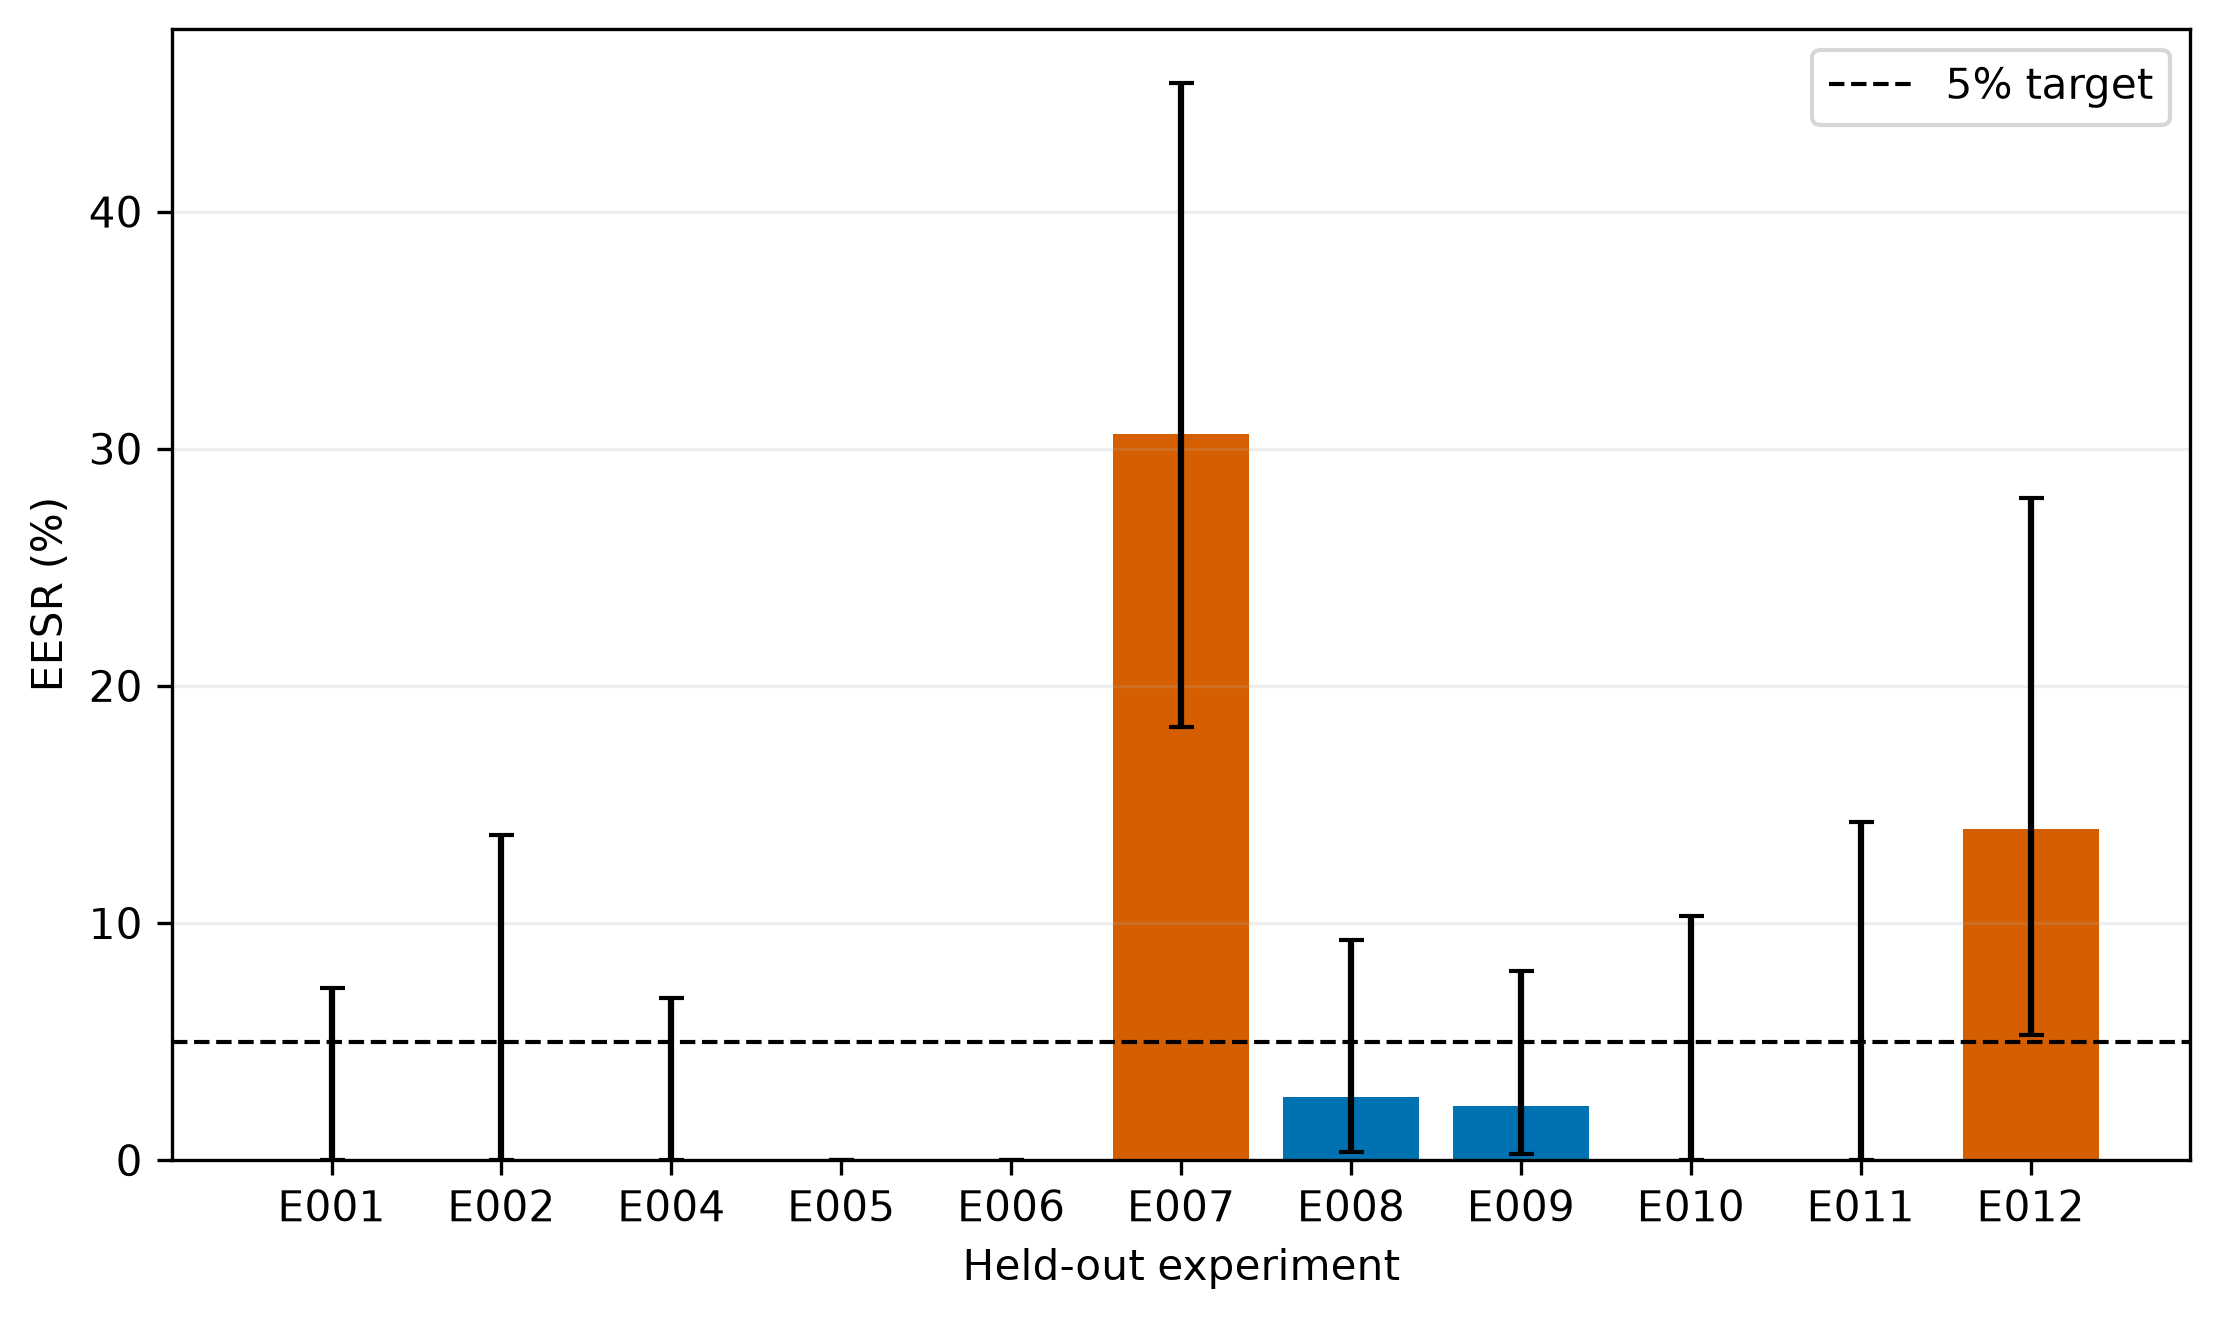
\includegraphics[width=\linewidth]{03_per_experiment_eesr.png}
    \caption{Observed EESR for each completely held-out experiment.}
  \end{subfigure}\hfill
  \begin{subfigure}[t]{0.49\textwidth}
    \centering
    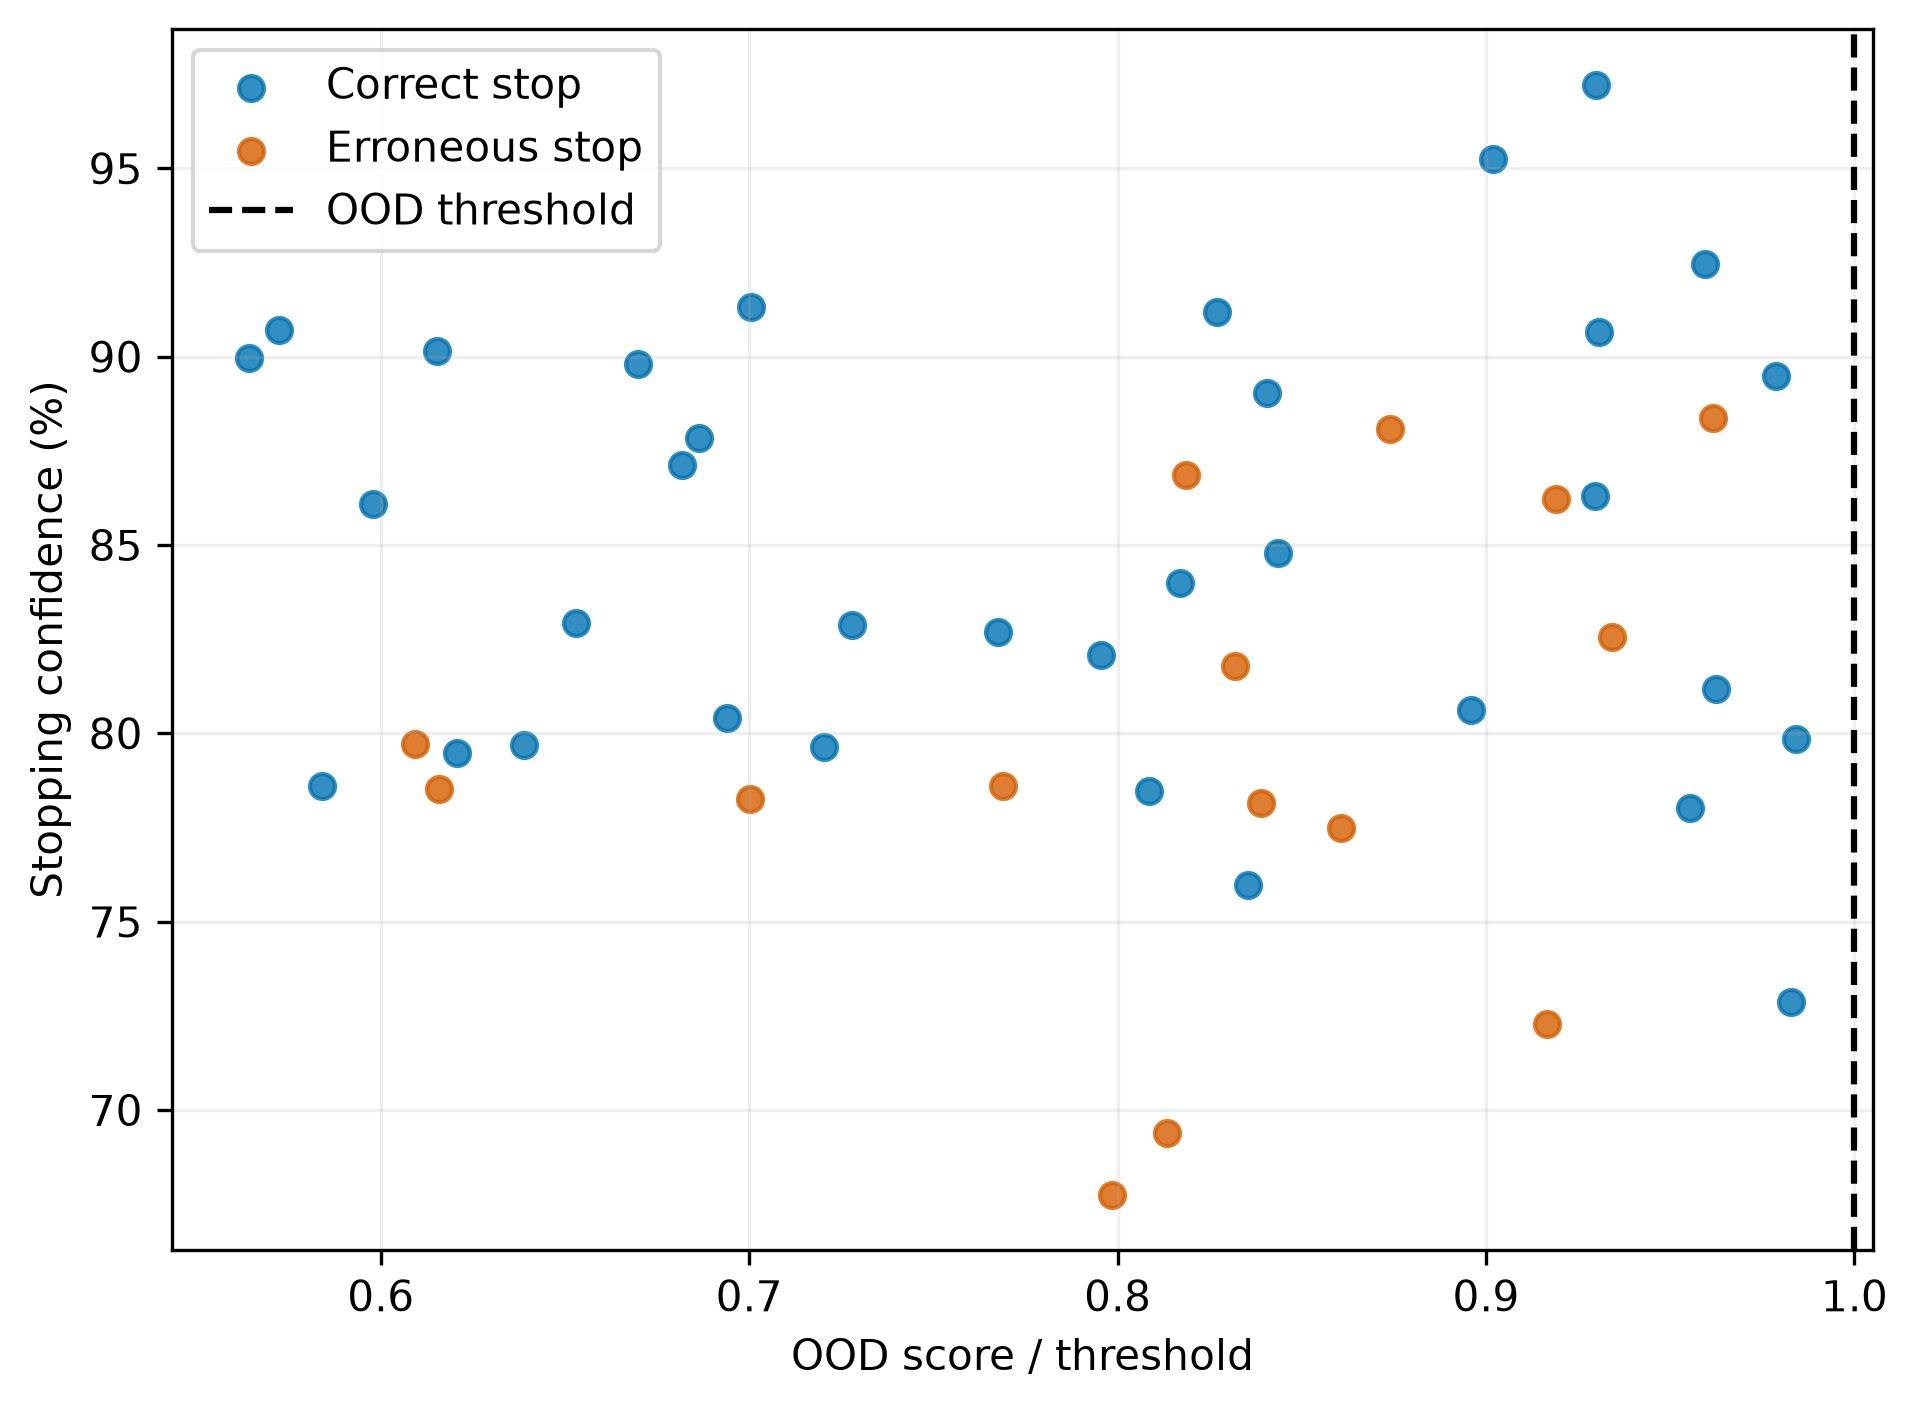
\includegraphics[width=\linewidth]{12_e007_failure_case.png}
    \caption{Decision-time evidence for the E007 failure case.}
  \end{subfigure}
  \caption{Experiment-level heterogeneity under the frozen 5\% RPE policy. Aggregate EESR was
  \pct{5.69}, but E007 reached \pct{30.61} among early stops and was not rejected by the frozen
  trajectory-level familiarity rule. This is a central limitation, not an excluded outlier.}
  \label{fig:heterogeneity}
\end{figure*}

\section{Robustness and negative results}

The primary policy did not remain below its target label under several perturbations
(\cref{tab:robustness}). Irregular sampling was particularly damaging, reaching \pct{10.61} EESR.
Feature noise, half-feature removal, and altered class balance produced \pct{7.37}, \pct{7.92},
and \pct{8.47}, respectively. Replacing the primary predictor with a decision tree produced
\pct{15.77}. Missing \pct{20} of observations produced \pct{6.16}, while reducing cadence to 2 h
produced \pct{5.64}. Transfer to the Lens endpoint failed at \pct{17.82} EESR with only \pct{6.43}
savings. These results are retained as evidence rather than treated as tuning opportunities.

\begin{table}[t]
\centering
\caption{Frozen robustness and negative-result summary.}
\label{tab:robustness}
\small
\begin{tabularx}{\columnwidth}{@{}>{\raggedright\arraybackslash}X rr@{}}
\toprule
Condition & EESR & Savings \\
\midrule
Primary RPE policy & 5.69\% & 12.26\% \\
Irregular sampling & 10.61\% & --- \\
0.25-SD feature noise & 7.37\% & --- \\
Half-feature removal & 7.92\% & --- \\
Altered class balance & 8.47\% & --- \\
Decision-tree predictor & 15.77\% & --- \\
20\% missing observations & 6.16\% & --- \\
2 h cadence & 5.64\% & --- \\
Lens endpoint transfer & 17.82\% & 6.43\% \\
\bottomrule
\end{tabularx}
\end{table}

\begin{figure*}[t]
  \centering
  \begin{subfigure}[t]{0.325\textwidth}
    \centering
    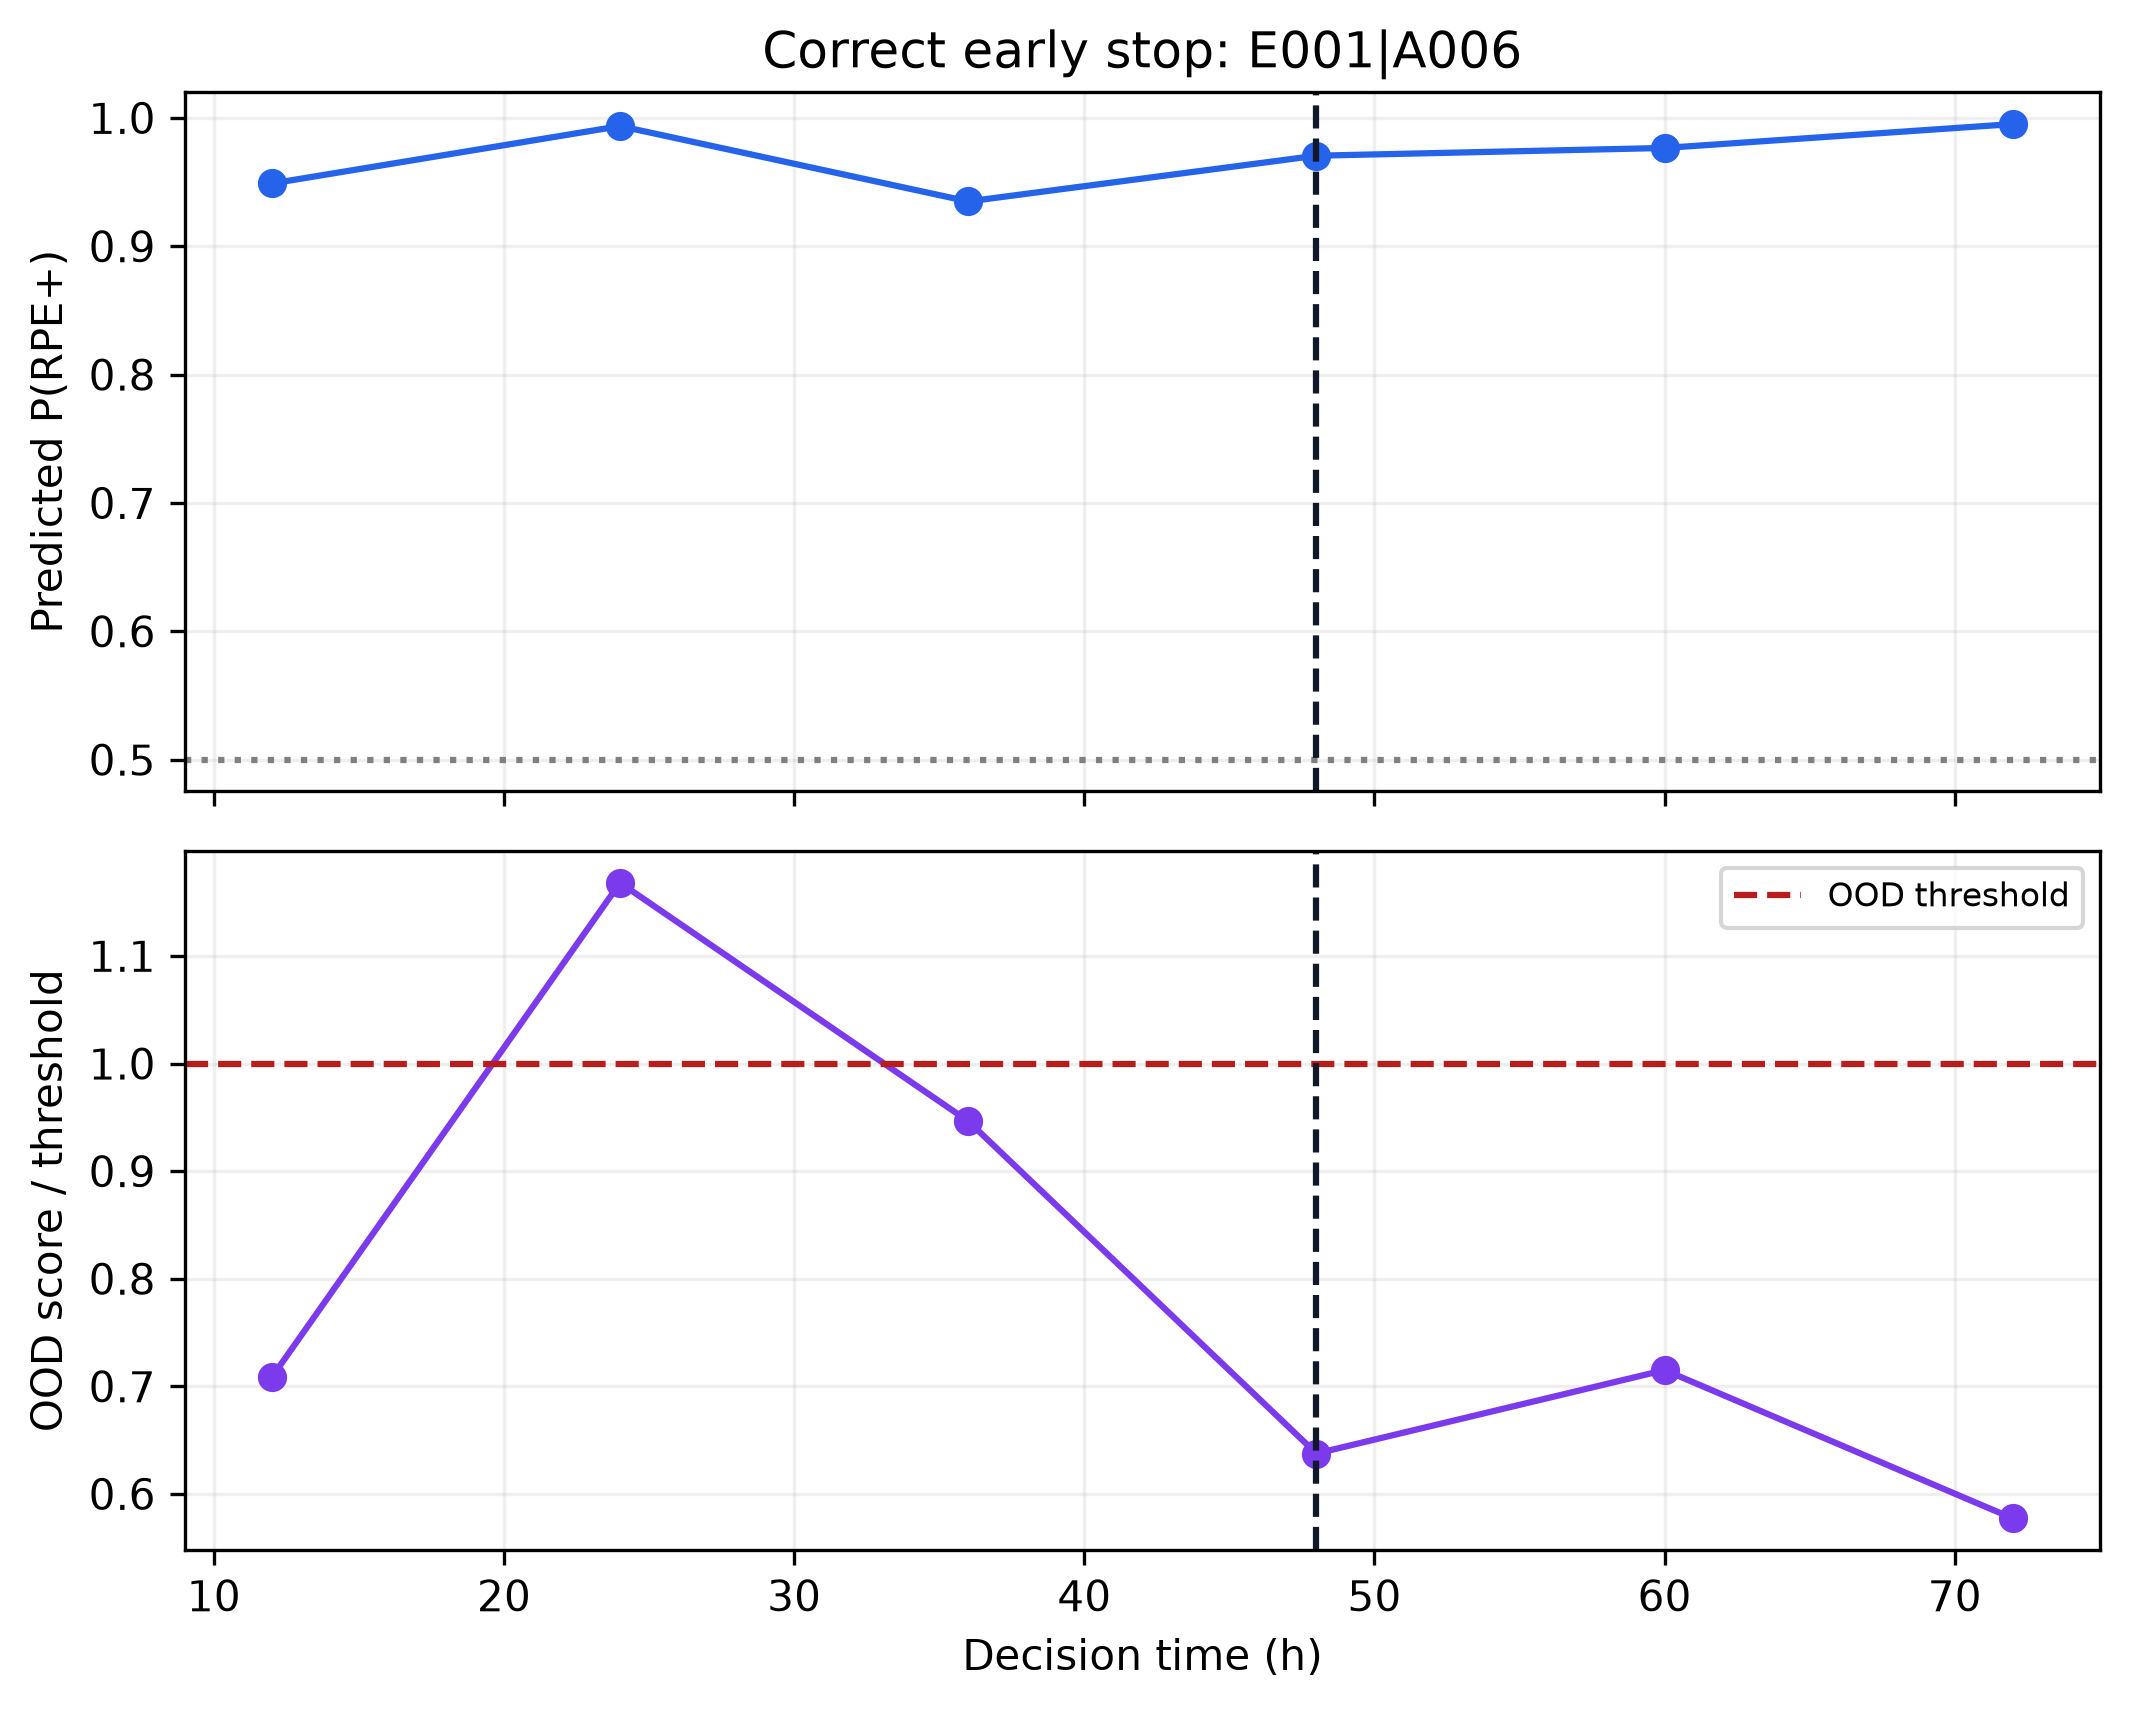
\includegraphics[width=\linewidth]{09_representative_successful_stop.png}
    \caption{Correct early stop.}
  \end{subfigure}\hfill
  \begin{subfigure}[t]{0.325\textwidth}
    \centering
    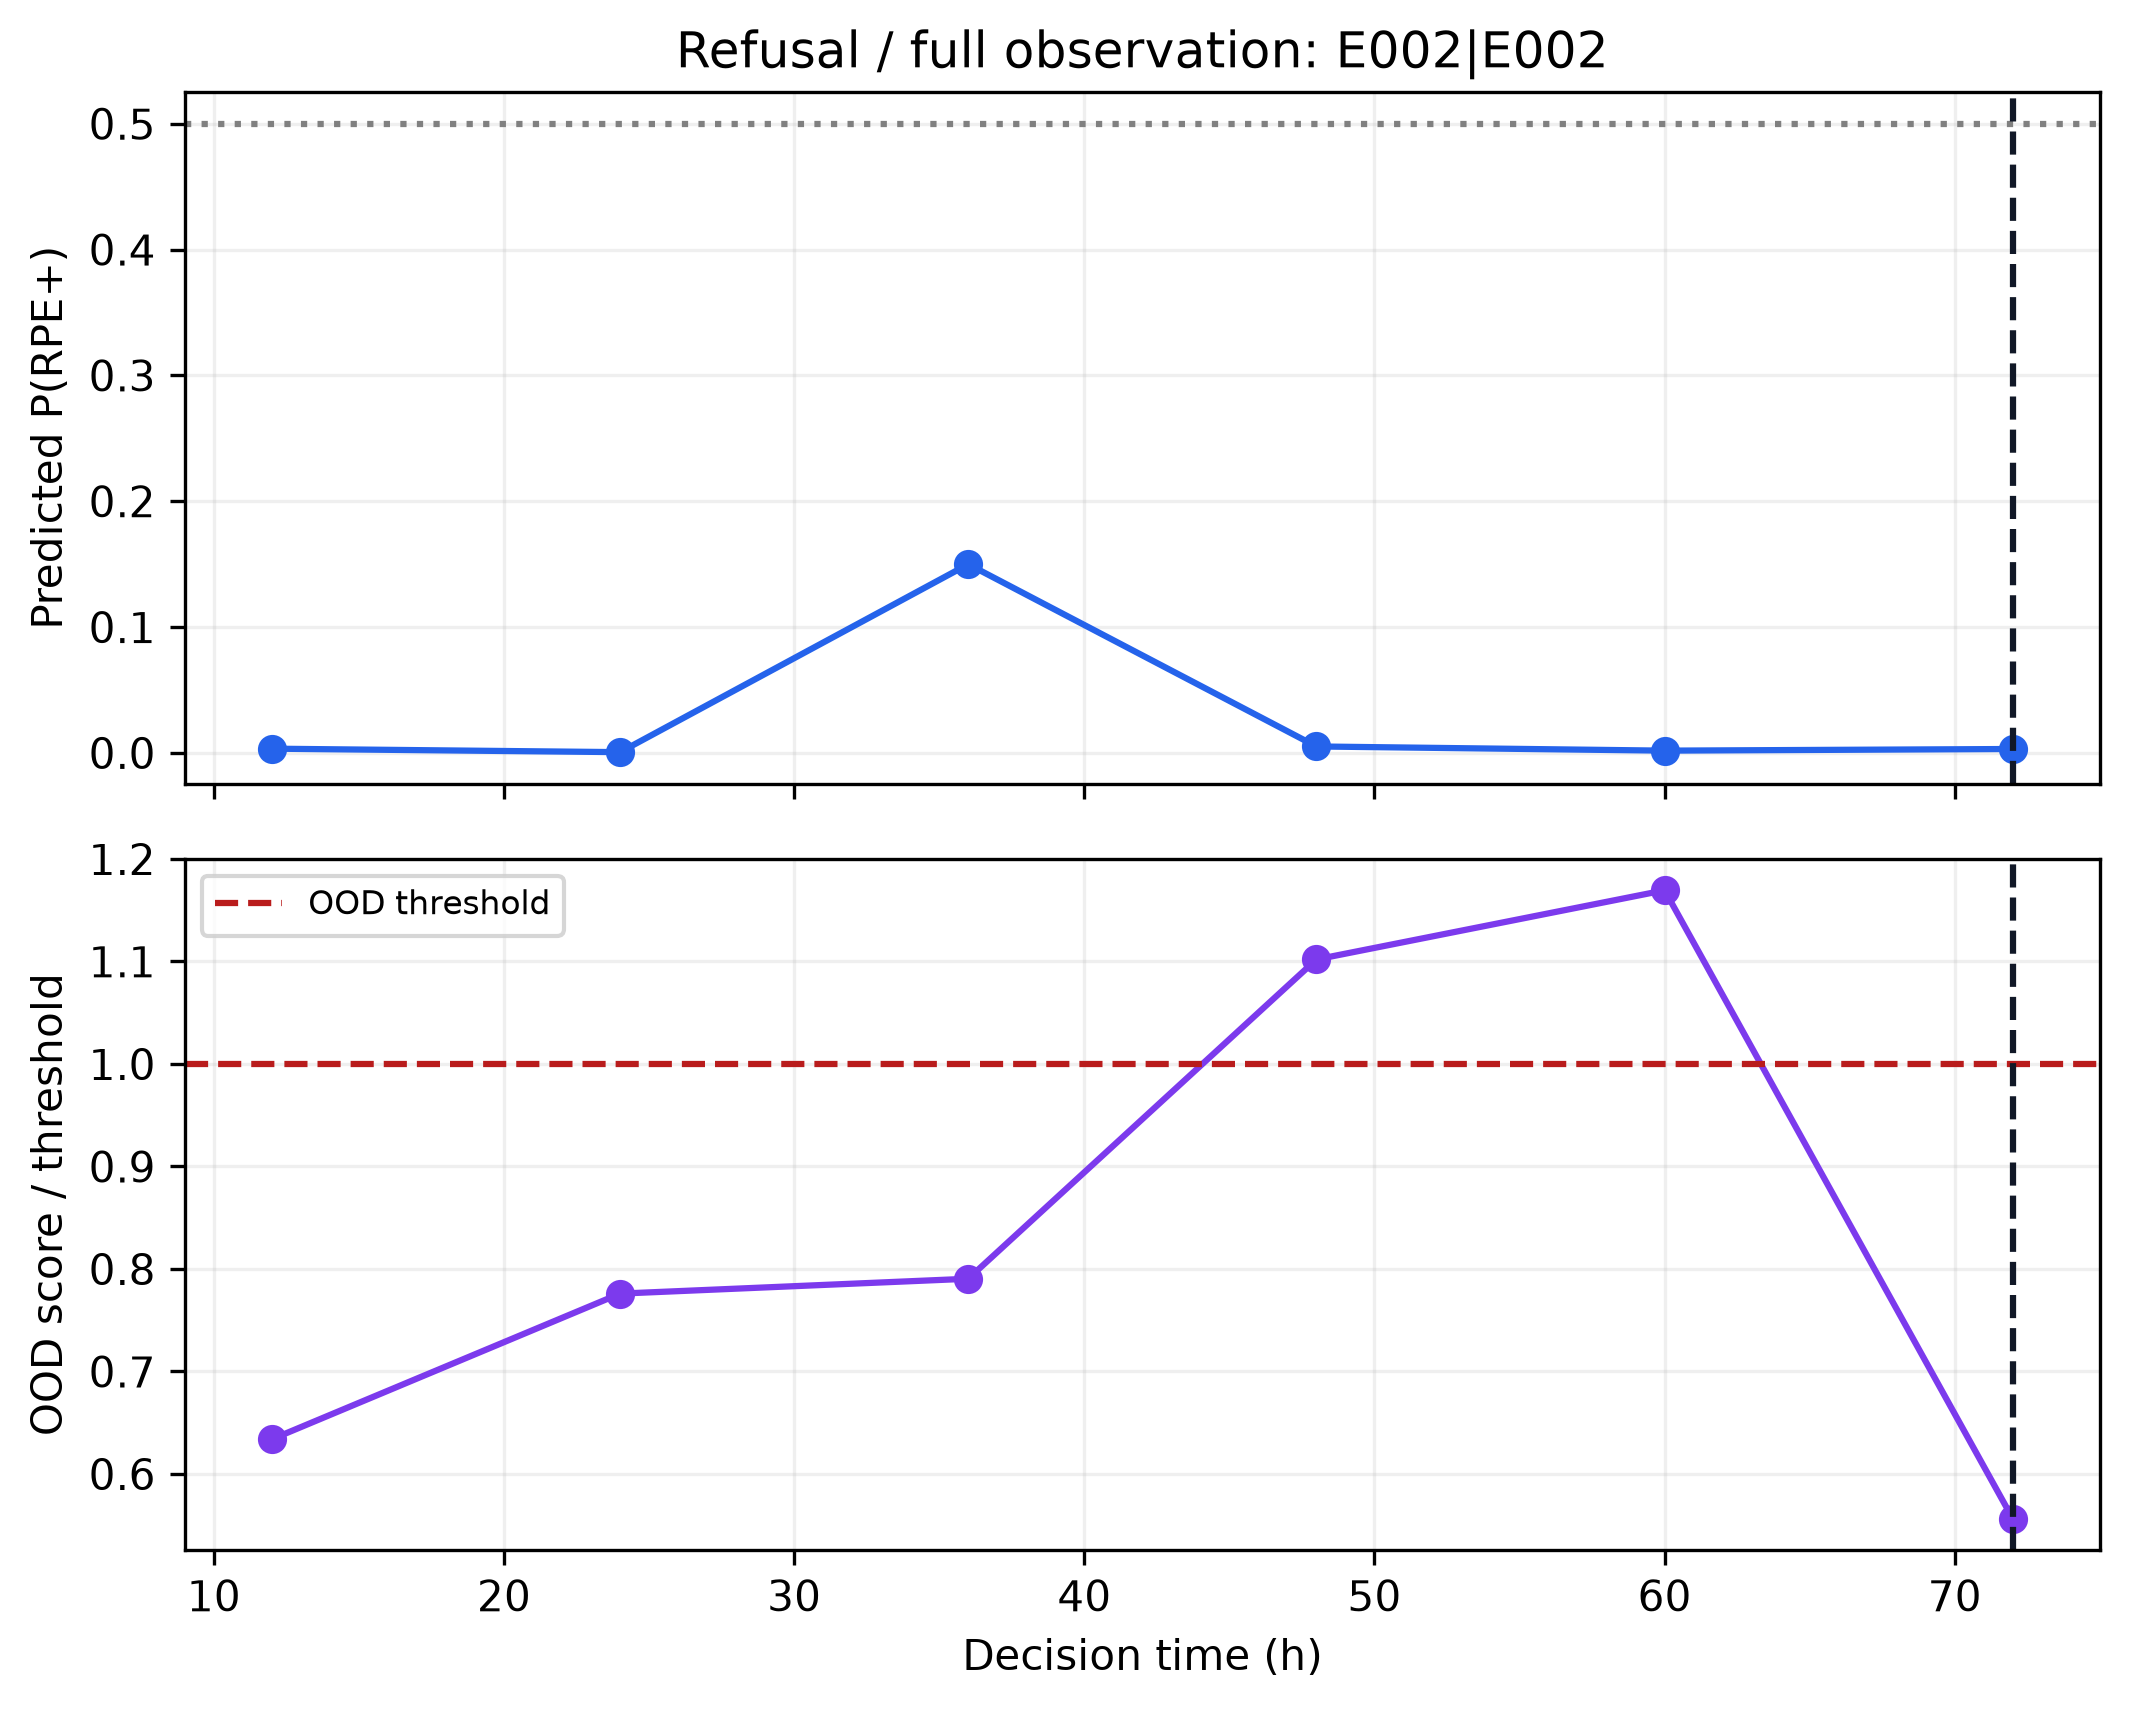
\includegraphics[width=\linewidth]{10_representative_abstention.png}
    \caption{Refused trajectory.}
  \end{subfigure}\hfill
  \begin{subfigure}[t]{0.325\textwidth}
    \centering
    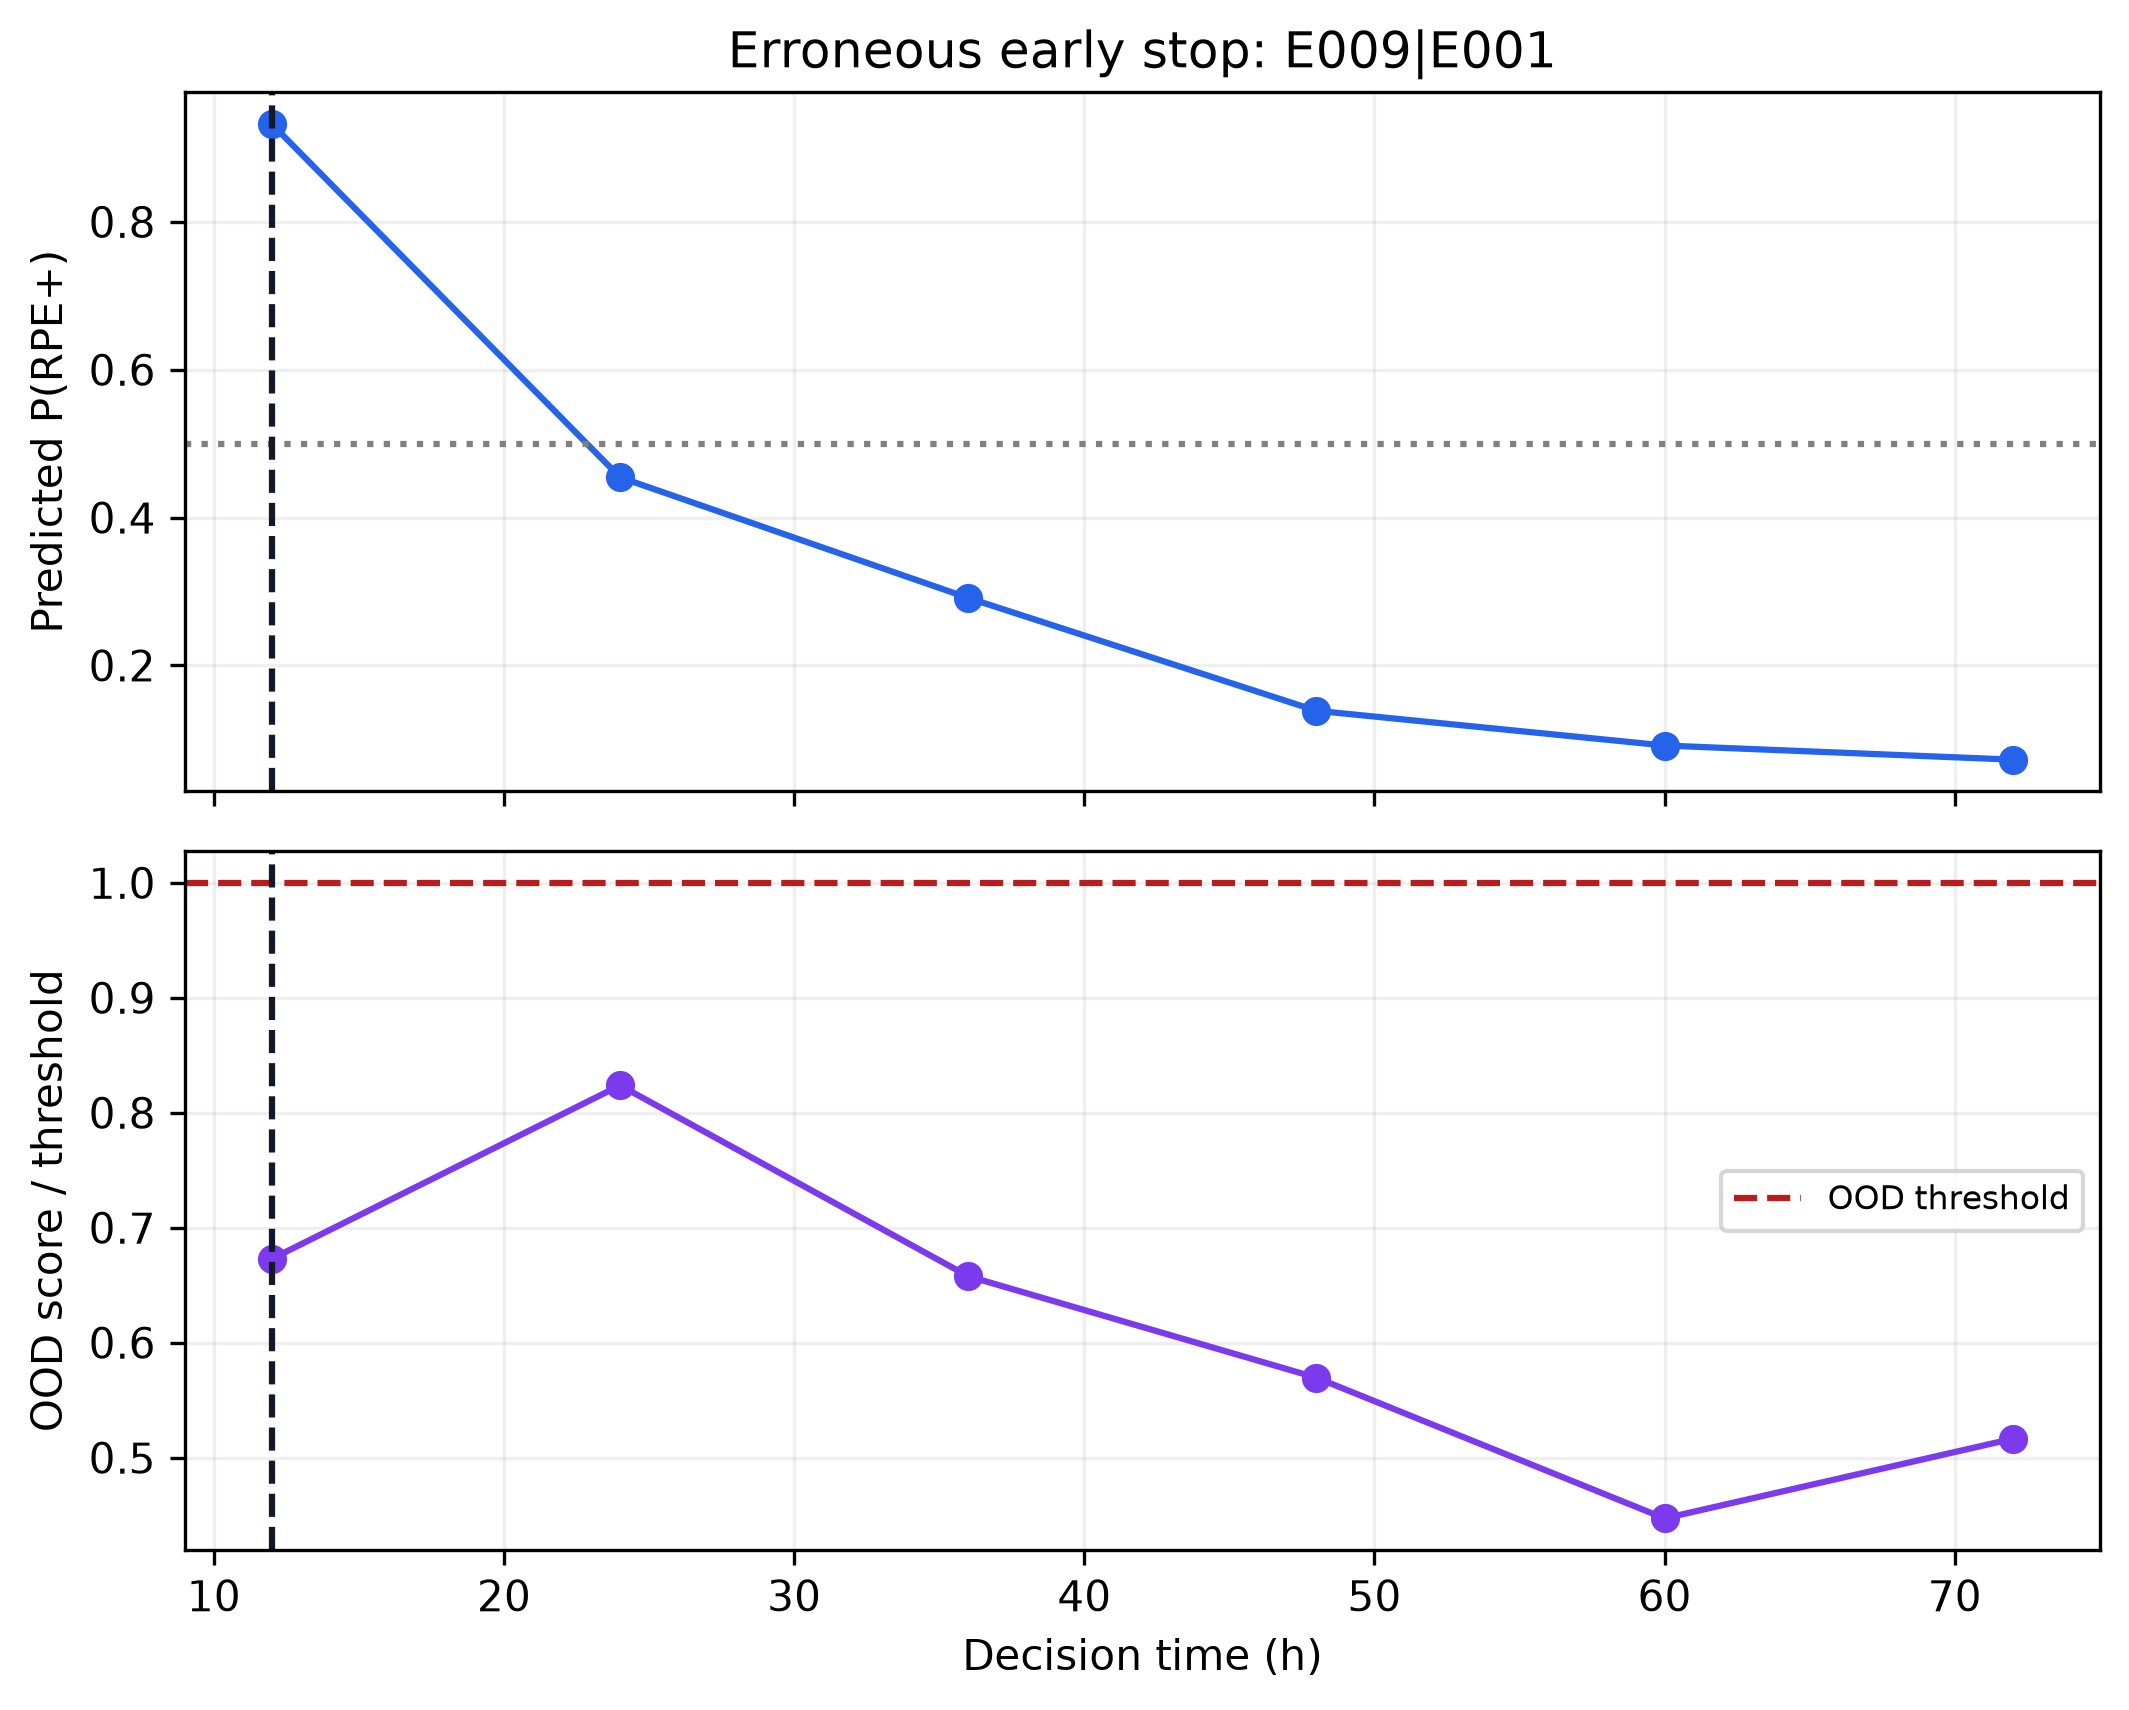
\includegraphics[width=\linewidth]{11_representative_erroneous_stop.png}
    \caption{Erroneous early stop.}
  \end{subfigure}
  \caption{Representative frozen held-out trajectories. The examples expose the intended decision
  contract: early automation when calibrated evidence passes, continued observation after refusal,
  and an explicit failure that remains in the audit record.}
  \label{fig:trajectories}
\end{figure*}

\section{Discussion}

\subsection{Early prediction is not safe termination}

The source study established that longitudinal morphology contains early endpoint information.
The present results show that converting such information into an intervention requires a distinct
evaluation. Full \method had lower observed EESR than the tested alternatives at its selected
operating point, but this improvement came with selective coverage. Its value lies in the ability
to continue or abstain when evidence does not pass, not in forcing every trajectory into an early
decision.

\subsection{What E007 teaches}

E007 demonstrates that acceptable aggregate performance can coexist with severe
experiment-specific failure. Whole-experiment separation reveals this failure but does not solve
it. The current feature-distance rule recognized some unfamiliar trajectories, yet E007's errors
were confidently inside its accepted region. A familiarity metric based on marginal feature
distance can miss conditional or calibration shift. Larger calibration populations and explicit
group-conditional validation are needed before intervention.

\subsection{Interpreting coverage and savings}

Coverage describes the fraction of units for which early automation is permitted at a particular
operating point. Lower coverage may be appropriate when the cost of a false stop is high. Likewise,
\pct{12.26} savings means that, in retrospective replay, scheduled observations after frozen
decision times would not have been required for early-stopped units. It does not establish a
\pct{12.26} reduction in experiment duration, instrument occupancy, labor, storage cost, or money.
Those consequences require prospective operational measurement.

\subsection{Exploratory experiment-level gate}

An optional extension summarized each experiment using information available by 12 h. At the 5\%
operating point, it refused E007 and E008, prevented 17 errors, reduced EESR to \pct{2.54}, and
retained \pct{7.88} savings. At 10\%, however, it accepted all seven unsafe experiments, refused
all four safe experiments, prevented no errors, and worsened EESR to \pct{16.34}. This instability
precludes including the gate in the principal method claim.

\section{Limitations and future work}

The evidence is retrospective and comes from one published medaka dataset with only 11 independent
experiments. There is no human-organoid, independent-laboratory, prospective, intervention,
deployment, or direct organ-on-chip validation. The exact unit-level interval does not capture all
between-experiment biological uncertainty. The refusal rule can miss conditional and calibration
failures. Coverage and refusal are class-asymmetric. The policy provides neither anytime-valid nor
distribution-free nor group-conditional control. No operational study has measured labor,
microscope, storage, duration, or cost savings.

The immediate next experiment is a preregistered prospective evaluation in independent
laboratories that preserves complete experiment boundaries and logs every candidate decision
without acting on it. Subsequent work should evaluate human organoids and direct organ-on-chip
trajectories, enlarge calibration populations, examine class-conditional reliability, strengthen
missingness and cadence robustness, and develop formal anytime-valid group-conditional control
before any stopping intervention.

\section{Reproducibility}

The public workflow pins the Zenodo record, filename, 400,059,241-byte file size, MD5, and SHA-256.
Protocols, seeds, and the software environment are frozen. Machine-readable artifacts include
per-unit terminal decisions, per-time predictions, exact and experiment-bootstrap intervals,
operating frontiers, robustness analyses, figure-source mappings, and release manifests. A clean
clone reproduces the evidence with the locked environment and a single task-runner command. The
interactive demonstration reads frozen evidence and does not retrain. The complete public release
is available at \href{https://github.com/Atharva12081/GATES}{github.com/Atharva12081/GATES}.

The v1 evidence audit contained an audit-only yes/no decoding defect in descriptive prevalence
metadata. V2 corrected that metadata. The headline tables were independently recomputed and
remained numerically unchanged; the method, frozen decisions, and principal result did not change.

\section{Conclusion}

Early prediction is not the same as safe early termination. \method shows how longitudinal
biological prediction can be recast as an experiment-disjoint selective decision that may stop,
continue, or refuse. On frozen held-out medaka organoid trajectories, refusal reduced observed
premature error while retaining measurable estimated savings, but experiment-level failures and
wide uncertainty remain. The contribution is therefore an auditable decision framework and a
transparent retrospective evaluation---not a guarantee of safe deployment.

\begin{thebibliography}{8}

\bibitem[Xing et~al.(2012)Xing, Pei, and Yu]{xing2012early}
Z.~Xing, J.~Pei, and P.~S. Yu.
\newblock Early classification on time series.
\newblock \emph{Knowledge and Information Systems}, 31:105--127, 2012.
\newblock \href{https://doi.org/10.1007/s10115-011-0400-x}{doi:10.1007/s10115-011-0400-x}.

\bibitem[Geifman and El-Yaniv(2019)]{geifman2019selectivenet}
Y.~Geifman and R.~El-Yaniv.
\newblock SelectiveNet: A deep neural network with an integrated reject option.
\newblock In \emph{Proceedings of the 36th International Conference on Machine Learning},
  volume~97, pages 2151--2159, 2019.

\bibitem[Angelopoulos and Bates(2023)]{angelopoulos2023gentle}
A.~N. Angelopoulos and S.~Bates.
\newblock A gentle introduction to conformal prediction and distribution-free uncertainty
  quantification.
\newblock \emph{Foundations and Trends in Machine Learning}, 16:494--591, 2023.

\bibitem[Angelopoulos et~al.(2024)Angelopoulos, Bates, Fisch, Lei, and Schuster]{angelopoulos2024crc}
A.~N. Angelopoulos, S.~Bates, A.~Fisch, L.~Lei, and T.~Schuster.
\newblock Conformal risk control.
\newblock In \emph{International Conference on Learning Representations}, 2024.

\bibitem[Liu et~al.(2026)]{liu2026cbes}
Liu et~al.
\newblock Confidence-bound early stopping of experiments with sequential calibration.
\newblock \emph{Chemical Engineering Research and Design}, 230:756--766, 2026.
\newblock \href{https://doi.org/10.1016/j.cherd.2026.05.013}{doi:10.1016/j.cherd.2026.05.013}.

\bibitem[Leek et~al.(2010)]{leek2010batch}
J.~T. Leek et~al.
\newblock Tackling the widespread and critical impact of batch effects in high-throughput data.
\newblock \emph{Nature Reviews Genetics}, 11:733--739, 2010.
\newblock \href{https://doi.org/10.1038/nrg2825}{doi:10.1038/nrg2825}.

\bibitem[Walsh et~al.(2021)]{walsh2021dome}
I.~Walsh et~al.
\newblock DOME: Recommendations for supervised machine learning validation in biology.
\newblock \emph{Nature Methods}, 18:1122--1127, 2021.
\newblock \href{https://doi.org/10.1038/s41592-021-01205-4}{doi:10.1038/s41592-021-01205-4}.

\bibitem[Afting et~al.(2026)]{afting2026orgainoid}
C.~Afting et~al.
\newblock A deep learning-based computational pipeline predicts developmental outcome in retinal
  organoids.
\newblock \emph{PLOS Biology}, 24:e3003597, 2026.
\newblock \href{https://doi.org/10.1371/journal.pbio.3003597}{doi:10.1371/journal.pbio.3003597}.

\end{thebibliography}

\clearpage
\appendix
\onecolumn
\renewcommand{\arraystretch}{1.30}

\section{Frozen protocol and decision semantics}

The frozen analysis evaluates the complete sequential policy, not isolated per-time classifiers.
For every held-out experiment, preprocessing statistics, predictor parameters, confidence
thresholds, and familiarity thresholds are estimated without access to any of its wells, frames,
or labels. Each well contributes one terminal record to aggregate evaluation. The same trajectory
cannot contribute to more than one train, calibration, or test role within a rotation.

\begin{table}[H]
\centering
\caption{Operational interpretation of the three terminal actions in the retrospective policy.}
\label{tab:actions}
\normalsize
\begin{tabularx}{\textwidth}{@{}l>{\raggedright\arraybackslash}p{0.27\textwidth}>{\raggedright\arraybackslash}X@{}}
\toprule
Action & Frozen rule & Evaluation consequence \\
\midrule
\stopstate & Confidence passes and the prefix remains inside the fitted familiarity boundary. &
The endpoint prediction is committed before 72 h; an incorrect label contributes one erroneous
early stop. \\
\continuestate & Available evidence does not pass the stopping rule. &
The next scheduled observation is consumed and the policy is evaluated again at a later candidate
time. \\
\abstainstate & The trajectory crosses the frozen feature-distance refusal threshold. &
Early automation is disabled for that unit and observation continues through the endpoint. \\
\bottomrule
\end{tabularx}
\end{table}

\begin{table}[H]
\centering
\caption{Protocol invariants applied to every experiment-held-out rotation.}
\label{tab:invariants}
\normalsize
\begin{tabularx}{0.96\textwidth}{@{}>{\raggedright\arraybackslash}p{0.24\textwidth}>{\raggedright\arraybackslash}X@{}}
\toprule
Invariant & Implementation consequence \\
\midrule
Complete-experiment separation & No well, frame, prefix, or endpoint from the test experiment is
used for preprocessing, fitting, calibration, or refusal-threshold selection. \\
Prefix-only information & Features at candidate time $t$ summarize only measurements available by
$t$; future observations and endpoint labels are excluded. \\
Identifier and availability exclusion & Experiment identifiers and observation-availability
variables are not predictor inputs. \\
One held-out terminal record & Each of the 988 wells contributes exactly one final action and, when
applicable, one early endpoint prediction. \\
Frozen empirical interpretation & The 5\% label is a calibration target; evaluation reports the
observed full-policy outcome rather than a certified guarantee. \\
\bottomrule
\end{tabularx}
\end{table}

\clearpage
\section{Per-experiment frozen results}

\Cref{tab:perexperiment} reports the complete held-out RPE results at the primary operating point.
The distribution is strongly heterogeneous: E005 and E006 have no early stops, seven experiments
have no erroneous early stop, and E007 dominates the aggregate error count. Reporting only the
pooled 25/439 result would obscure this structure.

\begin{table}[H]
\centering
\caption{Full \method\ at the frozen 5\% operating point for each completely held-out experiment.}
\label{tab:perexperiment}
\normalsize
\begin{tabular}{@{}lrrrrrr@{}}
\toprule
Experiment & Units & Early stops & Errors & EESR & Coverage & Savings \\
\midrule
E001 & 80 & 49 & 0 & 0.00\% & 61.25\% & 16.67\% \\
E002 & 92 & 25 & 0 & 0.00\% & 27.17\% & 4.53\% \\
E004 & 96 & 52 & 0 & 0.00\% & 54.17\% & 9.03\% \\
E005 & 92 & 0 & 0 & 0.00\% & 0.00\% & 0.00\% \\
E006 & 95 & 0 & 0 & 0.00\% & 0.00\% & 0.00\% \\
E007 & 93 & 49 & 15 & 30.61\% & 52.69\% & 30.29\% \\
E008 & 91 & 75 & 2 & 2.67\% & 82.42\% & 16.67\% \\
E009 & 90 & 88 & 2 & 2.27\% & 97.78\% & 27.22\% \\
E010 & 92 & 34 & 0 & 0.00\% & 36.96\% & 6.16\% \\
E011 & 90 & 24 & 0 & 0.00\% & 26.67\% & 8.89\% \\
E012 & 77 & 43 & 6 & 13.95\% & 55.84\% & 17.53\% \\
\midrule
All & 988 & 439 & 25 & 5.69\% & 44.43\% & 12.26\% \\
\bottomrule
\end{tabular}
\end{table}

\begin{figure}[H]
  \centering
  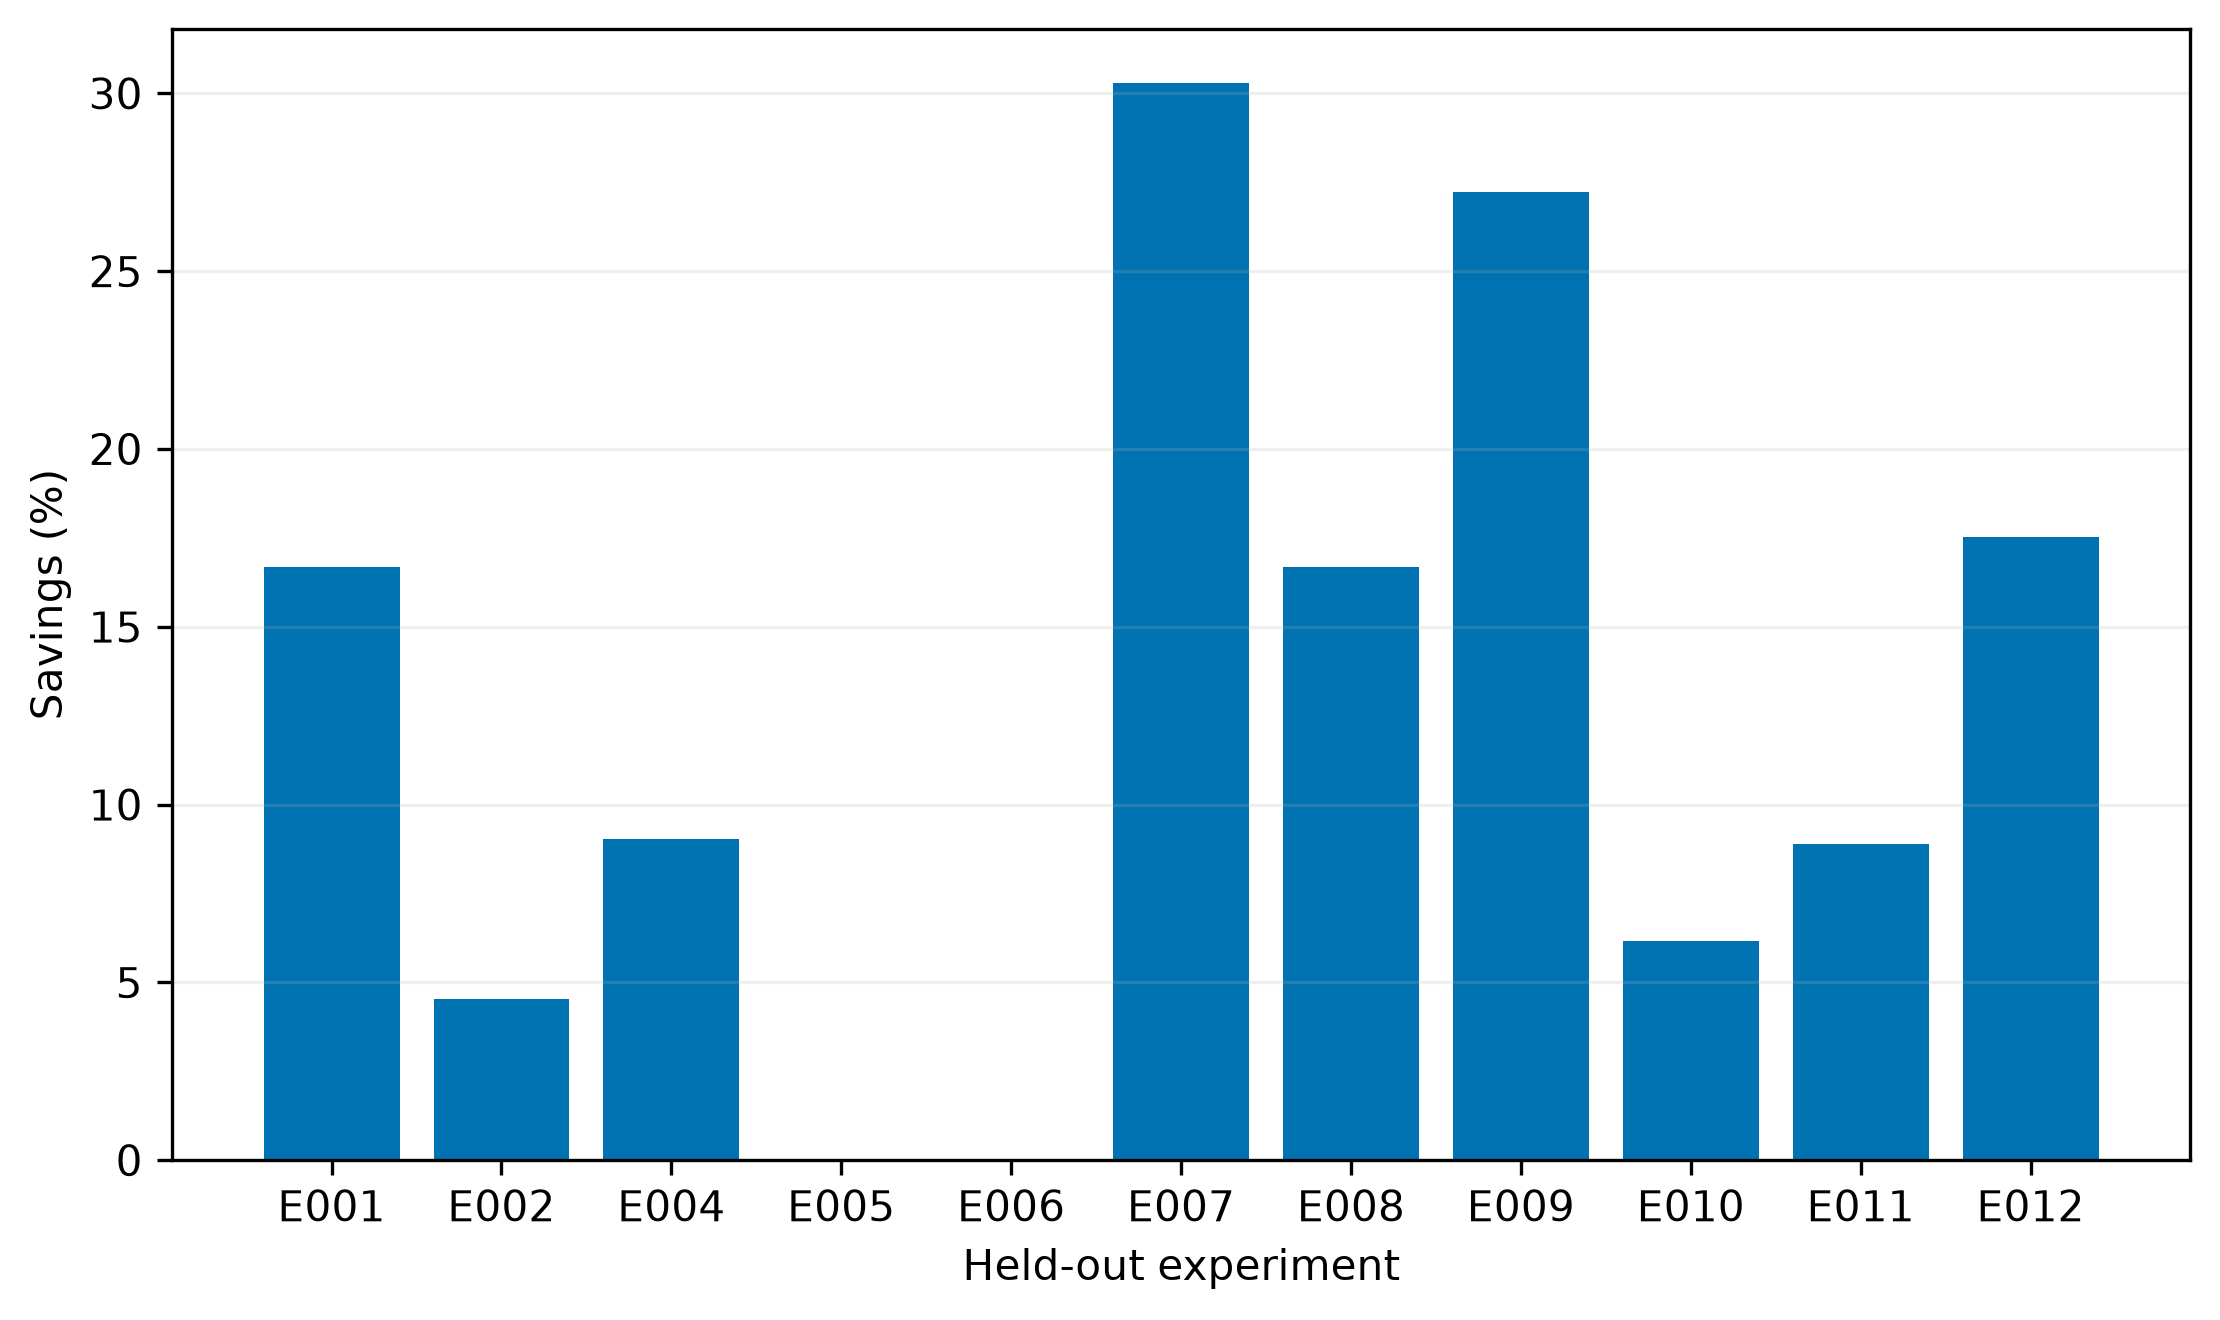
\includegraphics[width=0.96\textwidth]{04_per_experiment_observation_savings.png}
  \caption{Retrospectively estimated observation savings for each held-out experiment under the
  frozen 5\% policy. Savings and error vary together imperfectly: high estimated savings in E007
  coexist with severe premature error, reinforcing the need to report the complete tradeoff.}
  \label{fig:persavings}
\end{figure}

\clearpage
\section{Class-specific frozen-decision audit}

The class audit in \cref{tab:classaudit} is computed only from frozen unit decisions; no model,
threshold, split, or operating point was changed. Positive organoids were selected for early
stopping less often and refused more often. This asymmetry is a limitation and motivates larger
class-conditional calibration studies; it does not justify post hoc threshold adjustment.

\begin{table}[H]
\centering
\caption{Class-specific audit of frozen Full \method\ decisions at the 5\% operating point.}
\label{tab:classaudit}
\normalsize
\begin{tabular}{@{}lrrrrrrr@{}}
\toprule
Endpoint class & Units & Early stops & Coverage & Refusals & Refusal rate & Errors & EESR among stops \\
\midrule
RPE-negative & 583 & 295 & 50.60\% & 14 & 2.40\% & 15 FP & 5.08\% \\
RPE-positive & 405 & 144 & 35.56\% & 24 & 5.93\% & 10 FN & 6.94\% \\
\bottomrule
\end{tabular}
\end{table}

\section{Baseline and exploratory-gate details}

\begin{figure}[H]
  \centering
  \begin{subfigure}[t]{0.78\textwidth}
    \centering
    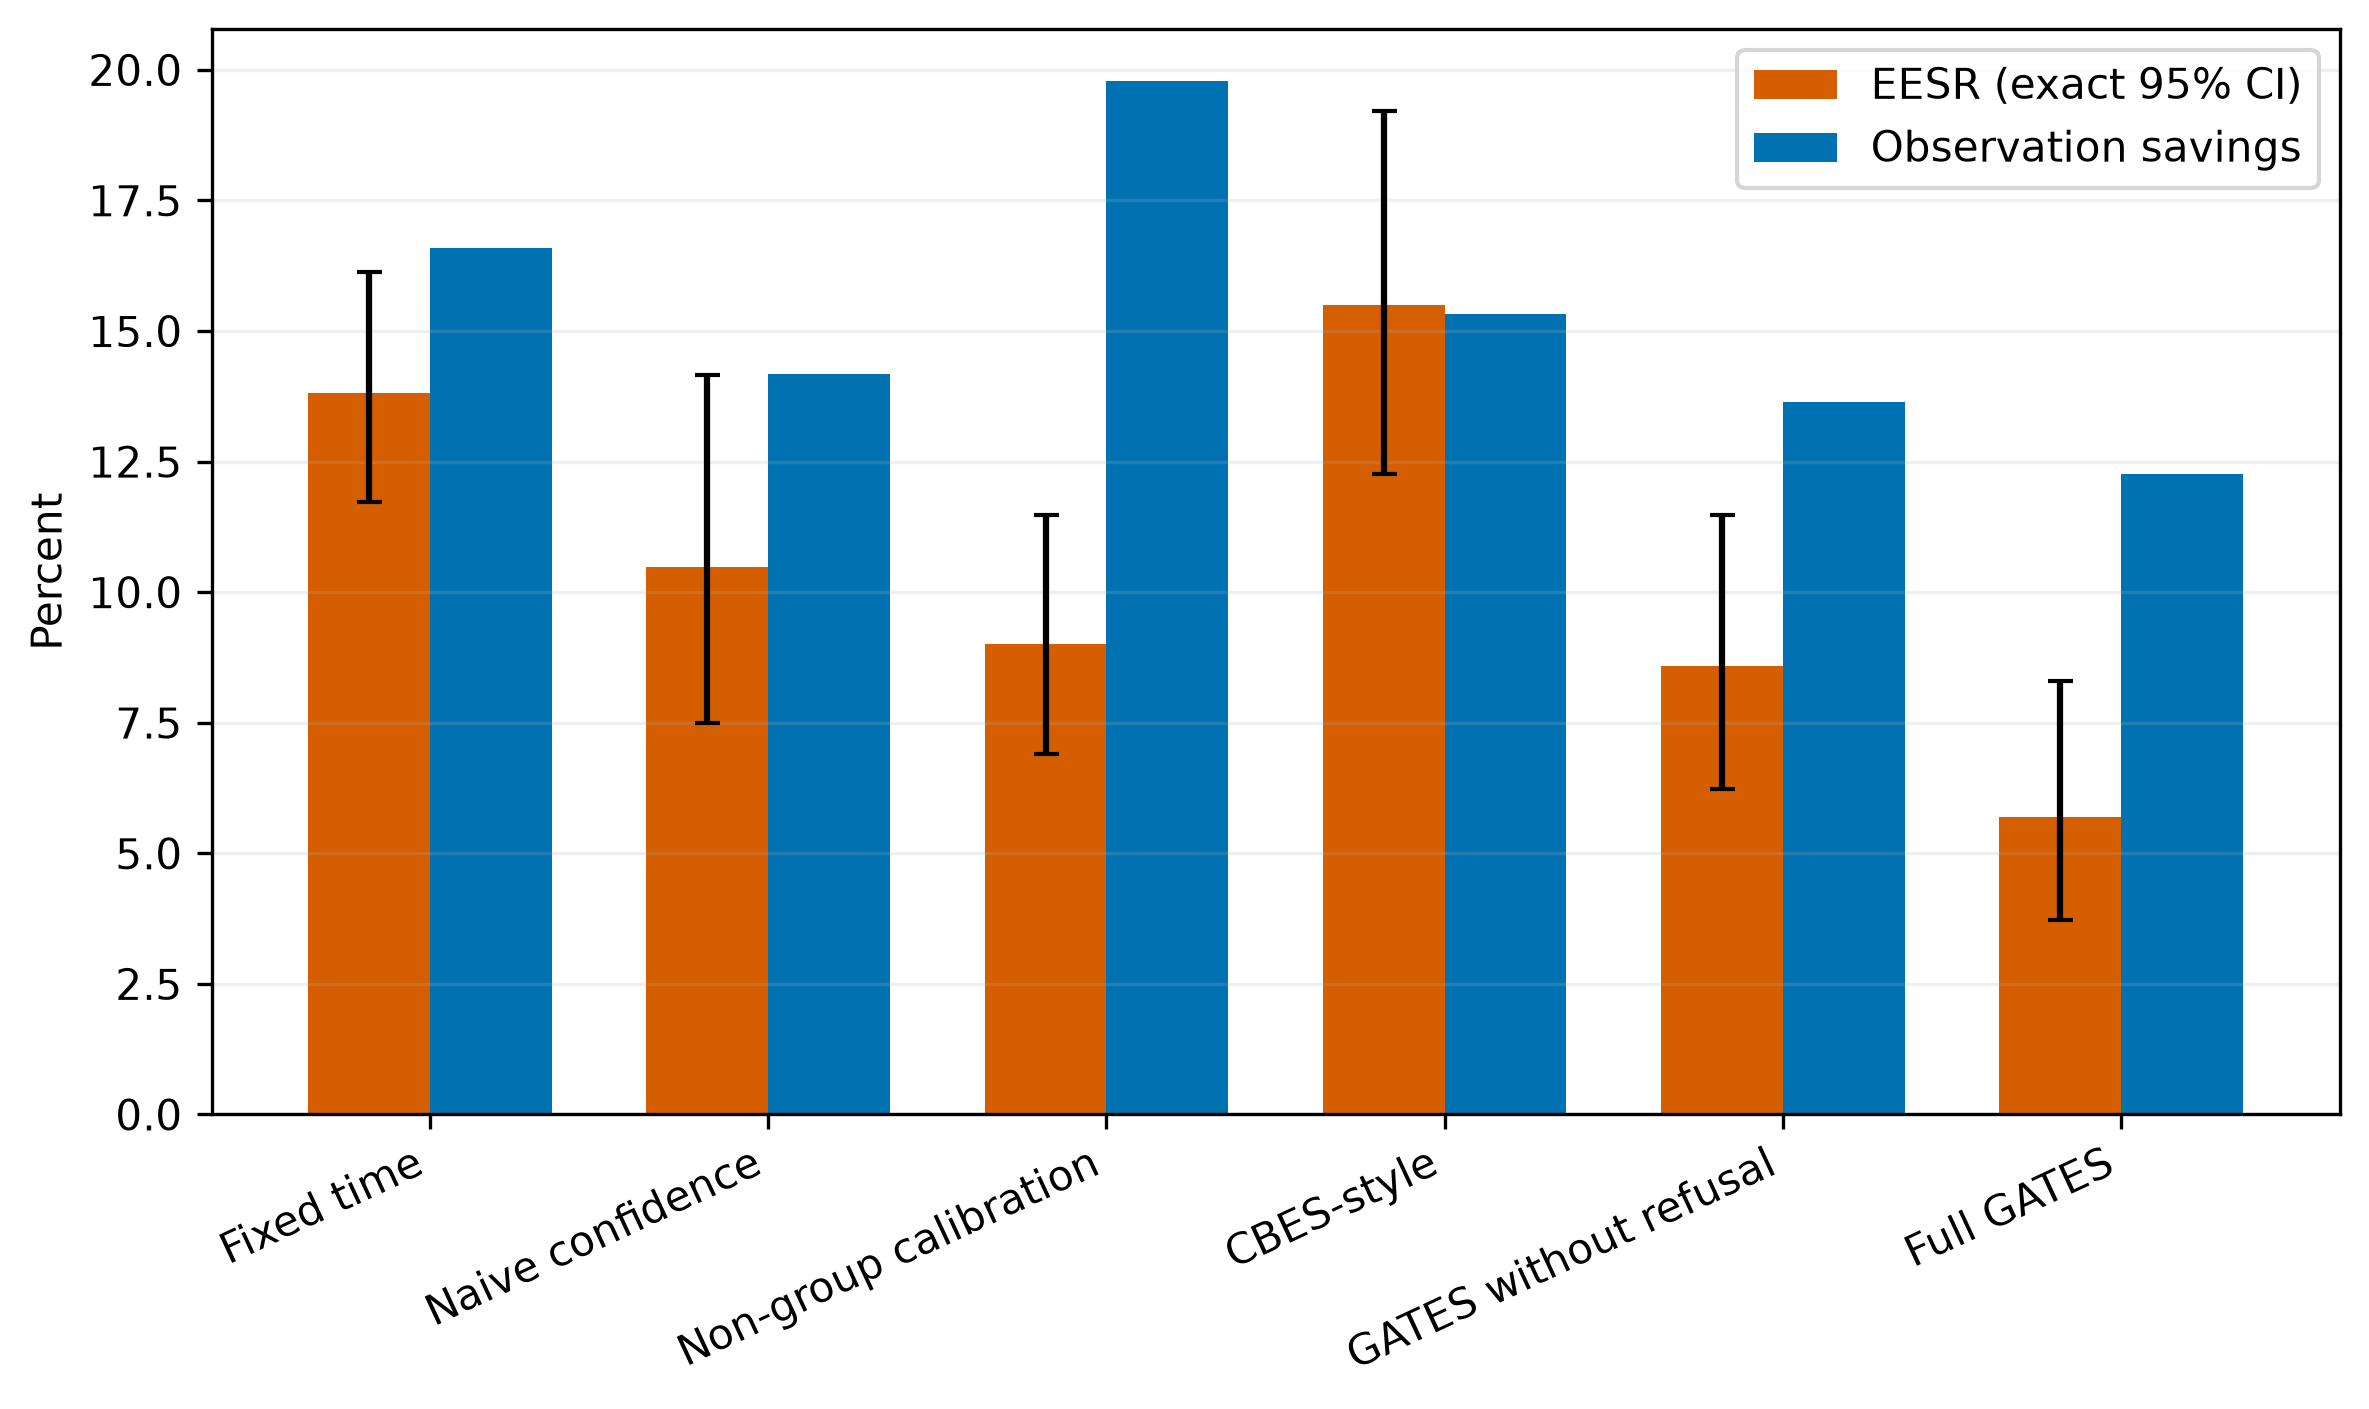
\includegraphics[width=\linewidth]{05_baseline_comparison_005.png}
    \caption{Method comparison at the 5\% operating-point label.}
  \end{subfigure}\par\vspace{5pt}
  \begin{subfigure}[t]{0.78\textwidth}
    \centering
    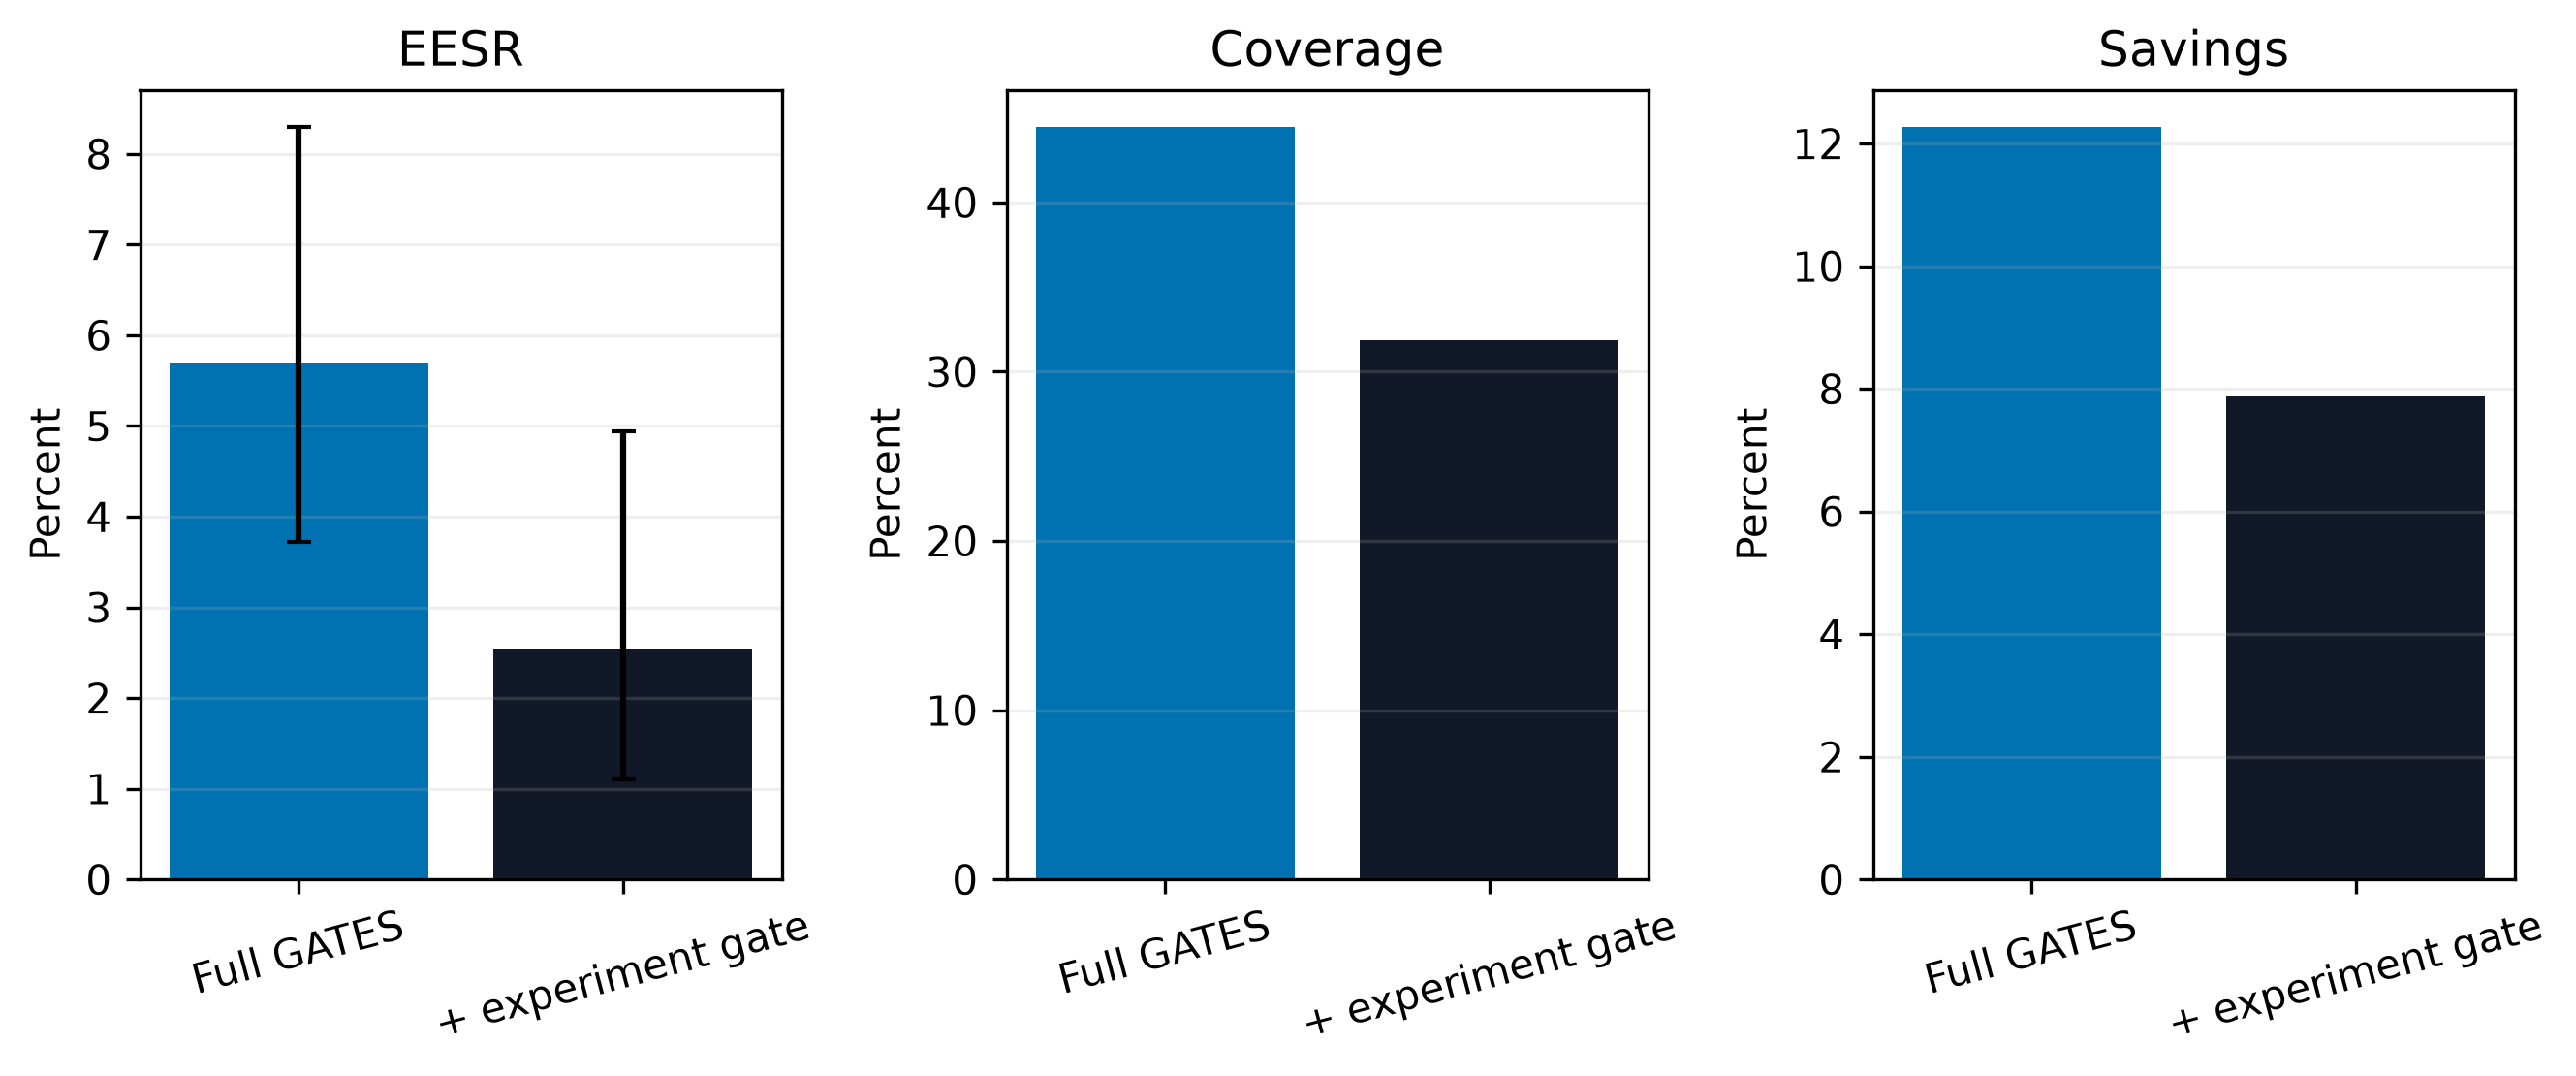
\includegraphics[width=\linewidth]{07_experiment_gate_005.png}
    \caption{Exploratory experiment gate at 5\%.}
  \end{subfigure}
  \caption{Supplementary comparisons from frozen evidence. The baseline panel complements the
  frontiers but does not equate methods with different coverage. The experimental gate helped at
  5\%, yet its instability at 10\% prevents promotion to the principal method.}
  \label{fig:suppcomparison}
\end{figure}

\clearpage
\begin{figure}[H]
  \centering
  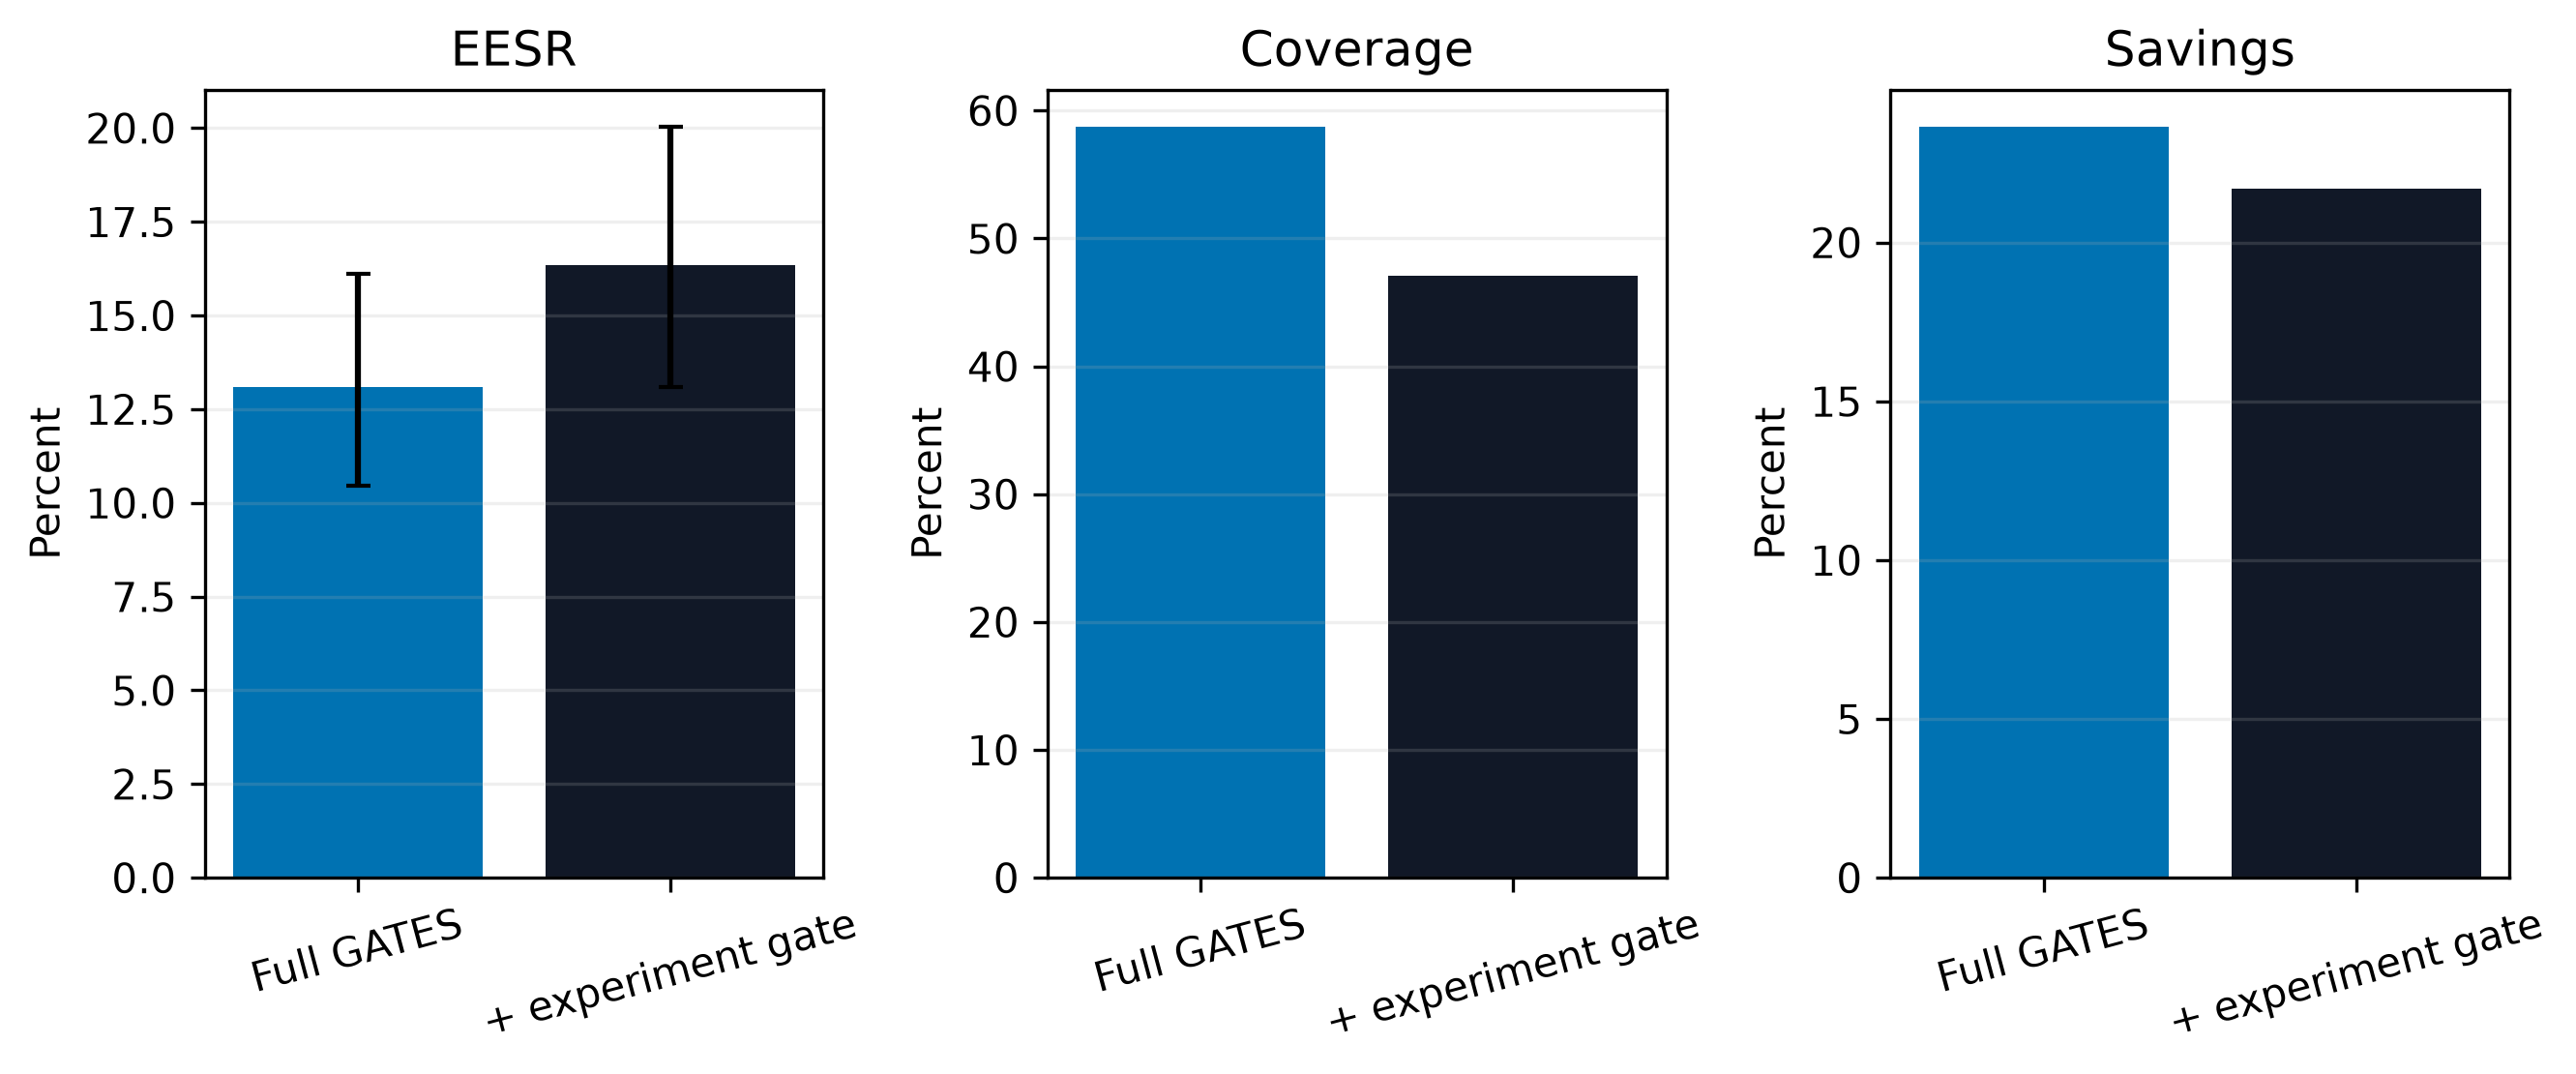
\includegraphics[width=0.96\textwidth]{08_experiment_gate_010.png}
  \caption{Failure of the exploratory experiment-level gate at the 10\% operating point. It
  accepted all seven unsafe experiments, refused all four safe experiments, prevented no errors,
  and produced \pct{16.34} EESR.}
  \label{fig:gatefailure}
\end{figure}

\begin{table}[H]
\centering
\caption{Exploratory experiment-level gate. This extension is not part of Full \method.}
\label{tab:expgate}
\normalsize
\begin{tabular}{@{}lrr@{}}
\toprule
Metric & 5\% target & 10\% target \\
\midrule
Early stops & 315 & 465 \\
Errors & 8 & 76 \\
EESR & 2.54\% & 16.34\% \\
Coverage & 31.88\% & 47.06\% \\
Savings & 7.88\% & 21.69\% \\
\bottomrule
\end{tabular}
\end{table}

\section{Uncertainty record}

\begin{table}[H]
\centering
\caption{Frozen headline estimates and uncertainty intervals. The exact interval conditions on
unit-level early stops; the experiment bootstrap resamples the 11 held-out experiments.}
\label{tab:uncertainty}
\normalsize
\begin{tabular}{@{}lrr@{}}
\toprule
Metric & Point estimate & Interval \\
\midrule
EESR & 5.69\% (25/439) & 3.72--8.29\% exact; 0.68--12.60\% experiment bootstrap \\
Coverage & 44.43\% (439/988) & 27.06--61.52\% experiment bootstrap \\
Observation savings & 12.26\% & 6.74--17.98\% experiment bootstrap \\
\bottomrule
\end{tabular}
\end{table}

The experiment-bootstrap intervals are the more relevant summary of between-experiment
generalization, although they remain imprecise with only 11 groups. Neither interval supplies a
prospective, anytime-valid, group-conditional, or distribution-free guarantee.

\clearpage
\section{Safety, reproducibility, and provenance}

\stopstate means that the frozen retrospective research rule passed; it does not prescribe
terminating a real experiment. \continuestate means that the stopping threshold has not passed.
\abstainstate disables early automation for a trajectory outside the fitted feature-distance
boundary and completes the 72 h protocol. Human oversight and prospective application-specific
validation remain mandatory.

The headline selector is the RPE dataset, aggregate experiment, Full \method, and 0.05 calibration
target in the frozen master evidence table. Figure-to-table mappings, source-data checksums,
decision records, and release hashes accompany the public repository. The retinal source data are
licensed CC BY 4.0; project code is released under the MIT License.

\begin{table}[H]
\centering
\caption{Reproducibility record included with the frozen release.}
\label{tab:repro}
\normalsize
\begin{tabularx}{\columnwidth}{@{}>{\raggedright\arraybackslash}X c@{}}
\toprule
Item & Status \\
\midrule
Pinned public source record and filename & Included \\
Byte size, MD5, and SHA-256 checks & Included \\
Locked dependency environment & Included \\
Frozen protocols and deterministic seeds & Included \\
Per-time predictions and per-unit decisions & Included \\
Figure-to-evidence mappings & Included \\
Release manifest and clean-clone replay & Included \\
Evidence-only interactive demonstration & Included \\
\bottomrule
\end{tabularx}
\end{table}

\subsection*{Requirements for a prospective study}

The present evidence supports a shadow-mode next step rather than autonomous stopping. A
preregistered evaluation should retain complete experiment boundaries, fit every calibration and
refusal parameter before test decisions are revealed, and log actions at every candidate time
without altering the experiment. Independent laboratories should be analyzed as distinct groups.
The study should report class-specific coverage and refusal, cadence and missingness behavior,
operational resource use, and every erroneous early stop. Human oversight remains necessary until
application-specific prospective evidence and a suitable formal risk-control procedure are
available. Human organoids and direct organ-on-chip trajectories require separate validation; the
medaka results do not establish performance in either setting.

\begin{table}[H]
\centering
\caption{Minimum evidence needed before considering an intervention study.}
\label{tab:prospective}
\normalsize
\begin{tabularx}{0.96\textwidth}{@{}>{\raggedright\arraybackslash}p{0.27\textwidth}>{\raggedright\arraybackslash}X@{}}
\toprule
Requirement & Purpose \\
\midrule
Preregistered frozen policy & Prevent threshold selection after viewing prospective outcomes. \\
Independent laboratories & Test transfer beyond the single released experimental source. \\
Shadow-mode sequential logging & Measure decisions prospectively without terminating acquisition. \\
Complete group separation & Preserve the biological generalization boundary. \\
Class-conditional reporting & Quantify asymmetric coverage, refusal, and error. \\
Operational measurements & Distinguish estimated observation savings from realized resource use. \\
Human oversight and stop rules & Protect experiments while evidence remains preliminary. \\
Direct target-system validation & Establish performance separately for human organoids or
organ-on-chip trajectories. \\
\bottomrule
\end{tabularx}
\end{table}

\end{document}
